% =====================================================================
% Viva preparation guide -- personal study document, NOT a graded deliverable.
%
% Compile:  xelatex VIVA_GUIDE.tex   (run twice for the table of contents)
%       or: bash docs/build_viva_guide.sh
%
% Needs a Devanagari-capable font (Nirmala UI on Windows, Noto Sans
% Devanagari elsewhere -- change the \newfontfamily line below).
%
% Every number here is also in report/final/final_report.pdf and is checked
% against the result artifacts by report/final/check_report_facts.py.
% =====================================================================
\documentclass[11pt]{report}

\usepackage[margin=1in]{geometry}
\usepackage{amsmath}
\usepackage{amssymb}
\usepackage{fontspec}
\usepackage{graphicx}
\usepackage{booktabs}
\usepackage{longtable}
\usepackage{array}
\usepackage{xcolor}
\usepackage{caption}
\usepackage{enumitem}
\usepackage{tikz}
\usetikzlibrary{arrows.meta,positioning,shapes.geometric,fit,backgrounds}
\usepackage[most]{tcolorbox}
\usepackage{titlesec}
\usepackage{fancyhdr}
\PassOptionsToPackage{hyphens}{url}
\usepackage[colorlinks=true,linkcolor=blue!50!black,urlcolor=blue!50!black,citecolor=blue!50!black]{hyperref}
\emergencystretch=3em
\sloppy

\newfontfamily\devanagarifont{Nirmala UI}
\newcommand{\dn}[1]{{\devanagarifont #1}}

% ---------------------------------------------------------------------
% Colours -- same palette as the Phase 1/2 learning guides.
% ---------------------------------------------------------------------
\definecolor{hindiblue}{HTML}{1F6F8B}
\definecolor{nepalipurple}{HTML}{7A4FA3}
\definecolor{conceptgreen}{HTML}{2E8B57}
\definecolor{warnred}{HTML}{C0392B}
\definecolor{examplegold}{HTML}{B8860B}
\definecolor{codegray}{HTML}{F5F5F5}
\definecolor{titlenavy}{HTML}{102A43}

\titleformat{\chapter}[display]
  {\normalfont\huge\bfseries\color{titlenavy}}
  {\chaptertitlename\ \thechapter}{18pt}{\Huge}
\titlespacing*{\chapter}{0pt}{-20pt}{18pt}
\titleformat{\section}
  {\normalfont\Large\bfseries\color{titlenavy}}{\thesection}{1em}{}
\titleformat{\subsection}
  {\normalfont\large\bfseries\color{hindiblue}}{\thesubsection}{1em}{}

\pagestyle{fancy}
\fancyhf{}
\fancyhead[L]{\small\textit{Viva Guide}}
\fancyhead[R]{\small\nouppercase{\leftmark}}
\fancyfoot[C]{\thepage}
\renewcommand{\headrulewidth}{0.4pt}

% ---------------------------------------------------------------------
% Callout boxes. The four that carry the answer structure are:
% shortans -> deeper -> example -> keypoint.
% ---------------------------------------------------------------------
\newtcolorbox{shortans}{colback=conceptgreen!6,colframe=conceptgreen,
  fonttitle=\bfseries,coltitle=white,colbacktitle=conceptgreen,
  title={\textbf{Short answer --- say this}},sharp corners=south,
  boxrule=1pt,left=2mm,right=2mm,breakable}

\newtcolorbox{deeper}{colback=hindiblue!6,colframe=hindiblue,
  fonttitle=\bfseries,coltitle=white,colbacktitle=hindiblue,
  title={\textbf{If the examiner asks for more}},sharp corners=south,
  boxrule=1pt,left=2mm,right=2mm,breakable}

\newtcolorbox{vexample}[1][Example]{colback=examplegold!8,colframe=examplegold,
  fonttitle=\bfseries,coltitle=white,colbacktitle=examplegold,
  title={\textbf{#1}},sharp corners=south,boxrule=1pt,left=2mm,right=2mm,breakable}

\newtcolorbox{keypoint}{colback=titlenavy!7,colframe=titlenavy,
  fonttitle=\bfseries,coltitle=white,colbacktitle=titlenavy,
  title={\textbf{Key point}},sharp corners=south,boxrule=1pt,
  left=2mm,right=2mm,breakable}

\newtcolorbox{trap}[1][Trap --- get ahead of this]{colback=warnred!8,colframe=warnred,
  fonttitle=\bfseries,coltitle=white,colbacktitle=warnred,
  left=2mm,right=2mm,title={\textbf{#1}},breakable}

\newtcolorbox{qabox}[1]{colback=nepalipurple!5,colframe=nepalipurple,
  fonttitle=\bfseries,coltitle=white,colbacktitle=nepalipurple,
  title={\textbf{Q: #1}},sharp corners=south,boxrule=1pt,left=2mm,right=2mm,
  breakable}

\newtcolorbox{notebox}[1][Note]{colback=gray!8,colframe=gray!60!black,
  fonttitle=\bfseries,left=2mm,right=2mm,title={\textbf{#1}},breakable}

\newtcolorbox{sayit}[1][Say it like this]{colback=conceptgreen!4,
  colframe=conceptgreen!70!black,fonttitle=\bfseries,left=2mm,right=2mm,
  title={\textbf{#1}},breakable}

% Shared TikZ vocabulary.
\tikzset{
  stage/.style  = {draw=black!55, rounded corners=2pt, fill=black!4,
                   inner sep=3pt, align=center, font=\footnotesize, minimum height=14pt},
  hstage/.style = {stage, fill=hindiblue!12, draw=hindiblue!70},
  lstage/.style = {stage, fill=nepalipurple!12, draw=nepalipurple!70},
  gstage/.style = {stage, fill=conceptgreen!12, draw=conceptgreen!70},
  flow/.style   = {-{Stealth[length=4pt]}, draw=black!60, line width=0.5pt},
}

\setlist[itemize]{topsep=2pt,itemsep=1pt,parsep=0pt,leftmargin=14pt}
\setlist[enumerate]{topsep=2pt,itemsep=1pt,parsep=0pt,leftmargin=16pt}

\title{\Huge\textbf{Viva Preparation Guide}\\[0.3cm]
\Large Two From-Scratch Monolingual Transformers\\[0.1cm]
\Large Hindi (Model H) and Nepali (Model L)\\[0.3cm]
\large Explaining, defending and deriving every part of the project}
\author{Swaraj Kumar\\[0.2cm]
\small \textit{Personal study document --- not a graded deliverable}}
\date{\today}

\begin{document}
\maketitle

\begin{tcolorbox}[colback=gray!8,colframe=gray!50!black,
  title={\textbf{What this document is, and how to use it}}]
This is my own preparation guide for the final viva. It is \textbf{not} a
course deliverable --- the graded report is
\texttt{report/final/final\_report.pdf}.

Every number in here is the same number as in that report, and both are
checked against the actual result files by
\texttt{report/final/check\_report\_facts.py}, which fails if a value drifts
away from the artifact it came from. It also verifies that every function and
class name cited here really exists in the repository.

\medskip
\textbf{How to use it.} Read Chapter~1 and the cheat sheet first, then work
through Chapters~3--5. Chapters~9, 10 and 11 --- design decisions, limitations
and trap questions --- are where examiners actually spend their time. Do not
memorise: the \emph{Think of it like this} boxes exist so that you can rebuild
an answer from understanding when the exact wording has gone.
\end{tcolorbox}

\tableofcontents

% =======================================================================
\chapter{The Two-Minute Introduction}
\chaptermark{Two-Minute Introduction}
% =======================================================================

\section{30-second version}

\begin{sayit}
I built two separate decoder-only Transformers from scratch in PyTorch, one
for Hindi and one for Nepali. Nothing is shared between them except the source
code --- separate corpora, separate tokenizers, separate weights. Both are
about 23 million parameters. The interesting result is that Hindi looks 41\%
better on perplexity, but that advantage mostly disappears when you measure in
bits-per-byte, because the two tokenizers chop text into different-sized
pieces.
\end{sayit}

\section{1-minute version}

\begin{sayit}
The task was to build two monolingual language models of about 25M parameters
each, with no pretrained weights and no pretrained tokenizers. I picked Hindi
as the higher-resource language and Nepali as the lower-resource one, and I
picked that pair deliberately because both use Devanagari --- if the script is
the same and the architecture is the same, then any difference between the
models has to come from the data or the tokenizer, not from the writing system
or model size.

\smallskip
Phase~1 was collecting and cleaning the corpora and training the tokenizers:
506 million Hindi tokens and 635 million Nepali, both with over 20\% manually
collected. Phase~2 was implementing the Transformer myself --- attention,
causal masking, positional embeddings --- and pretraining both models for about
475 million tokens on a Kaggle T4. Phase~3 was generating synthetic
comparative-reasoning data in each language and finetuning on it.

\smallskip
The headline results are that Hindi gets test perplexity 27.41 and Nepali
46.68, but on bits-per-byte it is 0.5382 against 0.4846 --- the ranking flips.
And in Phase~3, exact match went from 0\% to 35\%, but when I forced the models
to choose between the names in the question they were at chance, so they
learned the answer format rather than the comparison.
\end{sayit}

\section{2-minute version}

Say the one-minute version, then add:

\begin{sayit}[Add this for the two-minute version]
The part I would most want to talk about is that this project gave me the same
trap twice, in opposite directions. In Phase~2, if I had only reported
perplexity I would have concluded the low-resource model was far worse ---
bits-per-byte showed most of that gap was the tokenizer. In Phase~3, if I had
only reported exact match I would have concluded the models learned to reason
--- forced choice showed they had not. Both times a second metric measuring the
same thing in different units is what caught it.

\smallskip
I also traced two Phase~1 decisions forward. Nepali's tokenizer has no byte
fallback, which showed up as a column of zeros that I misread as a good score;
two phases later it meant the Nepali vocabulary had no Devanagari digit at all,
so 4.8\% of my generated reasoning data turned into unknown tokens. And Hindi
only deduplicates on exact SHA-1 hashes while Nepali does MinHash
near-duplicate removal plus train/test decontamination --- which is a real
weakness in the Hindi pipeline and a limit on how strongly I can interpret the
comparison.
\end{sayit}

\begin{keypoint}
Lead with the controlled-comparison design --- same script, same architecture.
That one sentence is what makes the whole project sound deliberate rather than
assembled.
\end{keypoint}

% =======================================================================
\chapter{The Complete Project Pipeline}
\chaptermark{Project Pipeline}
% =======================================================================

\section{The evidence chain}

Every stage below was run \textbf{twice and independently}, once per language.
Only the source code is shared.

\begin{figure}[htbp]
\centering
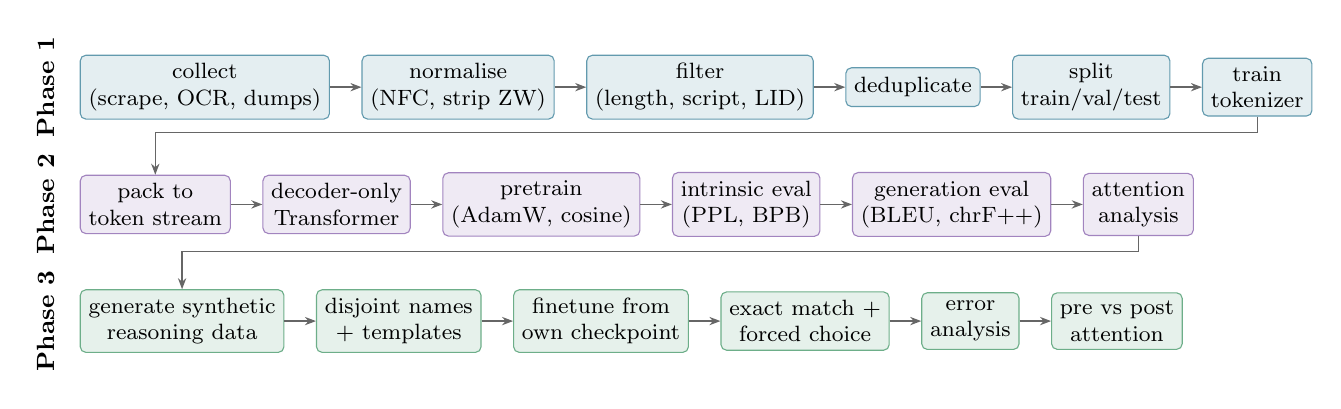
\begin{tikzpicture}[node distance=4mm]
\node[hstage] (c1) {collect\\(scrape, OCR, dumps)};
\node[hstage, right=of c1] (c2) {normalise\\(NFC, strip ZW)};
\node[hstage, right=of c2] (c3) {filter\\(length, script, LID)};
\node[hstage, right=of c3] (c4) {deduplicate};
\node[hstage, right=of c4] (c5) {split\\train/val/test};
\node[hstage, right=of c5] (c6) {train\\tokenizer};

\node[lstage, below=7mm of c1.south west, anchor=north west] (p1) {pack to\\token stream};
\node[lstage, right=of p1] (p2) {decoder-only\\Transformer};
\node[lstage, right=of p2] (p3) {pretrain\\(AdamW, cosine)};
\node[lstage, right=of p3] (p4) {intrinsic eval\\(PPL, BPB)};
\node[lstage, right=of p4] (p5) {generation eval\\(BLEU, chrF++)};
\node[lstage, right=of p5] (p6) {attention\\analysis};

\node[gstage, below=7mm of p1.south west, anchor=north west] (r1) {generate synthetic\\reasoning data};
\node[gstage, right=of r1] (r2) {disjoint names\\+ templates};
\node[gstage, right=of r2] (r3) {finetune from\\own checkpoint};
\node[gstage, right=of r3] (r4) {exact match +\\forced choice};
\node[gstage, right=of r4] (r5) {error\\analysis};
\node[gstage, right=of r5] (r6) {pre vs post\\attention};

\foreach \a/\b in {c1/c2, c2/c3, c3/c4, c4/c5, c5/c6, p1/p2, p2/p3, p3/p4,
                   p4/p5, p5/p6, r1/r2, r2/r3, r3/r4, r4/r5, r5/r6}
  \draw[flow] (\a) -- (\b);
\draw[flow] (c6.south) -- ++(0,-2mm) -| (p1.north);
\draw[flow] (p6.south) -- ++(0,-2mm) -| (r1.north);
\node[font=\small\bfseries, left=2mm of c1, rotate=90, anchor=south] {Phase 1};
\node[font=\small\bfseries, left=2mm of p1, rotate=90, anchor=south] {Phase 2};
\node[font=\small\bfseries, left=2mm of r1, rotate=90, anchor=south] {Phase 3};
\end{tikzpicture}
\caption{The two vertical arrows are the ones that carry Phase~1 decisions
into later measurements. Chapter~6 shows that both of them did.}
\end{figure}

\section{Every stage: what, why, how, output}

\begin{longtable}{@{}p{2.1cm}p{2.6cm}p{3.6cm}p{3.4cm}p{3.1cm}@{}}
\toprule
\textbf{Stage} & \textbf{What} & \textbf{Why} & \textbf{How} & \textbf{Output} \\
\midrule
\endfirsthead
\toprule
\textbf{Stage} & \textbf{What} & \textbf{Why} & \textbf{How} & \textbf{Output} \\
\midrule
\endhead
Collection & Gather raw text per language & Need $\approx$500M tokens, $\ge$20\% manual & Scraping, Wikipedia dumps, OCR, public corpora & 773,606 + 2,655,504 raw docs \\
Normalisation & Make text canonical & One string, two encodings defeats dedup & \texttt{normalize\_text()} --- four operations & Byte-canonical text \\
Filtering & Drop junk & Short, wrong-language or corrupt docs teach nothing & \texttt{devanagari\_ratio()}, \texttt{malformed\_ratio()}, \texttt{langdetect\_verdict()} & H: 704,103 docs kept \\
Dedup & Remove repeats & Duplicates inflate data and leak into test & H: \texttt{dedup\_key()}; L: \texttt{MinHasher} + LSH & H: 2,983; L: 2,350 + 49,734 \\
Splitting & Train/val/test & Need held-out data & Document-level, seeded & H 96/2/2, L 85/7.5/7.5 \\
Tokenizer & Text $\rightarrow$ IDs & Model works on IDs & SentencePiece on train split only & Unigram 8k, BPE 10k \\
Packing & Flatten to stream & Training reads contiguous windows & \texttt{CorpusPacker.pack\_split()} & 485,956,678 / 521,426,359 \\
Transformer & The model & The thing being built & \texttt{GPT} in \texttt{transformer.py} & 23.27M / 24.30M params \\
Pretraining & Learn the language & Next-token prediction & \texttt{Trainer.train()} & $\approx$475M tokens each \\
LM eval & Measure quality & PPL/BPB on held-out text & \texttt{perplexity\_and\_bpb()} & PPL 27.41 / 46.68 \\
Generation & Produce text & Check fluency, not just loss & \texttt{GPT.generate()} & chrF++ 16.29 / 18.05 \\
Attention & Inspect heads & I wrote attention, so I should inspect it & \texttt{summarise\_model\_attention()} & entropy 3.2047 / 3.0898 \\
Reasoning data & Synthetic task & Known ground truth, controlled leakage & \texttt{ReasoningGenerator} & 20k/2k/2k per language \\
Finetuning & Adapt to task & Learn task without destroying the LM & \texttt{FineTuner.train()} & best val at step 60 \\
Reasoning eval & Measure it & One metric is not enough & \texttt{ReasoningEvaluator} & EM 35.15/29.45\% \\
Error analysis & Explain failures & Accuracy hides the mechanism & \texttt{position\_analysis()} & middle-entity bias 72.6\% \\
\bottomrule
\end{longtable}

% =======================================================================
\chapter{Phase 1 --- Corpora and Tokenizers}
\chaptermark{Phase 1 --- Corpora and Tokenizers}
% =======================================================================

\section{Why these two languages?}

\begin{shortans}
Hindi as the higher-resource language because it has abundant public text, and
Nepali from the allowed lower-resource list. I chose that specific pair because
both are written in Devanagari --- if the script is held constant and I also
hold the architecture constant, then any gap between the models has to come
from data or tokenizer, not from the writing system or capacity.
\end{shortans}

\begin{deeper}
Bhojpuri was my original Model~L. I built the complete pipeline for it and it
passed validation, but public Bhojpuri text ran out at \textbf{84,217,032
tokens} --- only 16.8\% of the 500M target. The brief allows a documented
shortfall, but once the Nepali pipeline cleared its targets I switched rather
than submit a corpus one-sixth of the required size.
\end{deeper}

\begin{notebox}[Common follow-up]
\textit{``Isn't it a problem that they share a script?''} --- No, it is the
point. If they used different scripts I could never separate ``this script is
harder'' from ``this data is worse.''
\end{notebox}

\section{Manual versus downloaded data}

The brief required at least 20\% of final training tokens from manual
collection. Hindi came out at 30.66\% and Nepali at 26.41\%.

\begin{center}\small
\begin{tabular}{lrr}
\toprule
& \textbf{Model H (Hindi)} & \textbf{Model L (Nepali)} \\
\midrule
Manual tokens & 155,104,651 (30.66\%) & 167,787,251 (26.41\%) \\
Downloaded tokens & 350,747,377 & 467,417,082 \\
\textbf{Total} & \textbf{505,852,028} & \textbf{635,204,333} \\
\bottomrule
\end{tabular}
\end{center}

\textbf{Hindi manual sources:} self-extracted Wikipedia XML dump (66.7M), Gadya
Kosh prose (59.9M), patrika.com archive (19.5M), Kavita Kosh poetry (8.1M), 15
surviving archive.org items of 67 collected (0.85M). \textbf{Downloaded:}
FineWeb-2 \texttt{hin\_Deva} and four AI4Bharat Sangraha partitions.

\textbf{Nepali manual sources:} an \texttt{onlinekhabar} scrape (91.6\% of the
manual lane), a self-parsed Wikipedia dump, BBC Nepali, Wikibooks, Wiktionary,
Ekantipur, Ratopati, Nagarik, and OCR of archive.org books.
\textbf{Downloaded:} AI4Bharat Sangraha and IndicCorpV2.

\begin{deeper}
I quarantined the HuggingFace mirror of Hindi Wikipedia rather than using it,
because it is the same text as the dump I had already extracted --- counting
both would have double-counted. I also checked \texttt{robots.txt} per site
before scraping and recorded the verdict in
\texttt{scripts/manual\_sites.json}; bhaskar.com and amarujala.com disallow
automated access, so I did not scrape them.
\end{deeper}

\begin{trap}[Likely challenge --- raise it before they do]
\textit{``Is downloading a Wikipedia XML dump really manual collection?''}

\medskip
\textbf{Say:} ``I counted it as manual because I downloaded the raw dump and ran
the extraction and cleaning myself, rather than pulling a prepared corpus. I
can see the argument that it is closer to a download. If you exclude it, my
Hindi manual share drops from 30.66\% to \textbf{17.47\%}, which would be below
the floor --- so it is the single assumption my Phase~1 compliance rests on.''

\medskip
Saying this before they say it is far stronger than being caught by it.
\end{trap}

\section{Cleaning and normalisation}

\begin{figure}[htbp]
\centering
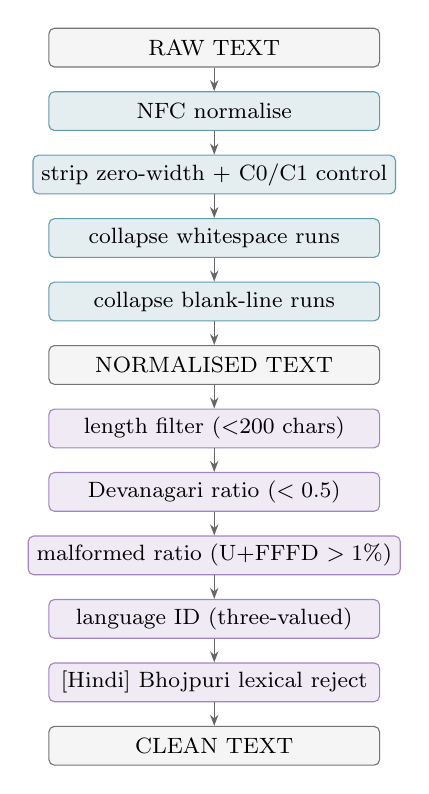
\begin{tikzpicture}[node distance=3mm, every node/.style={font=\footnotesize}]
\node[stage, minimum width=42mm] (a) {RAW TEXT};
\node[hstage, below=of a, minimum width=42mm] (b) {NFC normalise};
\node[hstage, below=of b, minimum width=42mm] (c) {strip zero-width + C0/C1 control};
\node[hstage, below=of c, minimum width=42mm] (d) {collapse whitespace runs};
\node[hstage, below=of d, minimum width=42mm] (e) {collapse blank-line runs};
\node[stage, below=of e, minimum width=42mm] (f) {NORMALISED TEXT};
\node[lstage, below=of f, minimum width=42mm] (g) {length filter ($<$200 chars)};
\node[lstage, below=of g, minimum width=42mm] (h) {Devanagari ratio ($<0.5$)};
\node[lstage, below=of h, minimum width=42mm] (i) {malformed ratio (U+FFFD $>1\%$)};
\node[lstage, below=of i, minimum width=42mm] (j) {language ID (three-valued)};
\node[lstage, below=of j, minimum width=42mm] (k) {[Hindi] Bhojpuri lexical reject};
\node[stage, below=of k, minimum width=42mm] (l) {CLEAN TEXT};
\foreach \x/\y in {a/b,b/c,c/d,d/e,e/f,f/g,g/h,h/i,i/j,j/k,k/l} \draw[flow] (\x) -- (\y);
\end{tikzpicture}
\caption{The cleaning pipeline. The first five boxes are
\texttt{normalize\_text()} in \texttt{scripts/clean\_lib.py}; the rest are
independent filters.}
\end{figure}

\begin{vexample}[A document going through normalisation]
\begin{tabbing}
\hspace{2.2cm}\=\kill
Raw: \> \dn{नमस्ते\quad\quad दुनिया} followed by three newlines, plus a stray U+200E \\[2pt]
\> $\downarrow$\; NFC compose \\
\> $\downarrow$\; strip U+200E (left-to-right mark) \\
\> $\downarrow$\; collapse the run of spaces to one \\
\> $\downarrow$\; collapse three newlines to a paragraph break \\[2pt]
Clean: \> \dn{नमस्ते दुनिया}
\end{tabbing}
\textbf{What changed and why:} the invisible direction mark is gone --- it
carries no meaning here and would make two otherwise identical documents hash
differently. The extra spacing is normalised so formatting variants collide
during deduplication.
\end{vexample}

\subsection{Why NFC and not NFKC?}

\begin{shortans}
NFC is canonical composition --- it picks one byte representation for strings
that are semantically identical. NFKC goes further and applies
\emph{compatibility} mappings, which actually change characters. I only want to
canonicalise, not to rewrite the text.
\end{shortans}

\begin{deeper}
NFKC would fold ligatures and alter some presentation forms. In Devanagari that
risks destroying information I want the model to learn. NFC is the safe choice:
same visible text, one canonical encoding.

\medskip
\textbf{Why it matters specifically here:} the same Devanagari string can be
stored two different ways. If I do not normalise before hashing, those two
forms produce different hashes, both survive deduplication, and I end up with
duplicates I believe I removed. NFC is therefore not cosmetic --- it is a
\textbf{precondition for deduplication working at all}.
\end{deeper}

\begin{keypoint}
NFC = same text, one encoding. NFKC = possibly different text. I needed the
first.
\end{keypoint}

\subsection{Zero-width characters, ZWNJ and ZWJ}

\begin{shortans}
I strip U+200E, U+200F, U+FEFF and the C0/C1 control range, but I deliberately
\textbf{keep} ZWNJ (U+200C) and ZWJ (U+200D).
\end{shortans}

\begin{deeper}
In Devanagari, ZWNJ and ZWJ change what is actually rendered --- they control
whether consonants form a conjunct ligature or stay separate. Removing them
would silently change the word. The others (direction marks, byte-order mark)
carry no linguistic content in this corpus and only create spurious hash
differences.
\end{deeper}

\begin{notebox}[Think of it like this]
A byte-order mark is \emph{packaging}. A ZWNJ is \emph{spelling}.
\end{notebox}

\subsection{Language identification}

\begin{shortans}
\texttt{langdetect\_verdict()} returns \textbf{three} values --- True, False, or
\texttt{None} for ``cannot tell'' --- with a minimum probability of 0.85. A
document is only dropped on a confident False, never on uncertainty.
\end{shortans}

\begin{deeper}
Treating ``undetermined'' as ``wrong language'' would throw away short or
unusual-but-valid documents. Nepali uses a fastText model
(\texttt{lid.176.bin}) with its own protections in
\texttt{nepali/scripts/corpuslib/langid.py}: \texttt{LanguageIdentifier} calls
the raw binding directly, runs \texttt{self\_test()} on known
Hindi/Nepali/English strings at construction, and raises if the error rate
crosses a threshold.
\end{deeper}

\begin{trap}[Worth volunteering --- a silent failure I found and fixed]
An earlier Nepali run was destroyed in exactly this area. The \texttt{fasttext}
wheel calls \texttt{np.array(probs, copy=False)}, which raises on NumPy $\ge$2.
Every prediction threw, the caller swallowed it as ``not our language'', and
millions of documents were deleted \emph{while the stage logged SUCCESS}. I
noticed because the surviving fraction was 5.85\%, and it was exactly the one
source configured to skip language ID.

\medskip
That is why the current code bypasses the broken wrapper, self-tests at
construction, and counts errors separately from rejections.
\textbf{Lesson:} a bare \texttt{except Exception} around a classifier turns a
library bug into silent data loss.
\end{trap}

\section{Deduplication --- exact versus near}

\begin{trap}[Know this cold --- the two pipelines are different]
\textbf{Do not say ``I used MinHash'' as a project-wide statement.} It is false
for Hindi, and an examiner who opens \texttt{scripts/clean\_lib.py} will find
out.
\end{trap}

\begin{center}\small
\begin{tabular}{lp{5.1cm}p{5.1cm}}
\toprule
& \textbf{Model H (Hindi)} & \textbf{Model L (Nepali)} \\
\midrule
Method & SHA-1 over normalised text (\texttt{dedup\_key()}) & exact \texttt{doc\_id}, then MinHash + LSH \\
Catches & exact copies, whitespace and punctuation variants & the above \textbf{plus} near duplicates \\
Removed & 2,983 (0.4\%) & 2,350 exact + 49,734 near \\
Decontamination & \textbf{none} & 17,111 train docs removed, rescan clean \\
\bottomrule
\end{tabular}
\end{center}

\begin{shortans}
Hindi deduplicates with a SHA-1 hash of the normalised, punctuation-stripped,
case-folded text. That catches exact copies and formatting variants but by
construction cannot catch two documents that say the same thing in different
words. Nepali uses MinHash with LSH and additionally decontaminates train
against validation and test.
\end{shortans}

\begin{trap}[The honest admission --- prepare it word for word]
``Hindi having no near-duplicate removal and no decontamination is a real
weakness. It means Hindi's test set may overlap its training data in ways
Nepali's cannot, and since the direction of that bias flatters Hindi, part of
the perplexity gap I attribute to tokenizer granularity could be unmeasured
leakage. I did not quantify it. It is the first thing I would fix.''
\end{trap}

\section{Shingles, Jaccard, MinHash and LSH}

Work through this until you can reproduce it on paper.

\begin{vexample}[Jaccard similarity by hand]
\begin{tabbing}
\hspace{1.6cm}\=\kill
Doc A: \> ``the cat is sitting on the mat'' \\
Doc B: \> ``the cat is sitting on a mat''
\end{tabbing}

Using \textbf{word} shingles of size 3 (my code uses 5-\emph{character}
shingles; words are easier to show):

\begin{tabbing}
\hspace{1.6cm}\=\kill
A: \> \{the cat is, cat is sitting, is sitting on, sitting on the, on the mat\} \\
B: \> \{the cat is, cat is sitting, is sitting on, sitting on a,\;\; on a mat\}
\end{tabbing}

\[
|A \cap B| = 3, \qquad |A \cup B| = 7, \qquad
J(A,B) = \frac{3}{7} = 0.43
\]

A and B have \emph{completely different} SHA-1 hashes but are 43\% similar ---
a near duplicate that exact matching silently keeps.
\end{vexample}

\begin{enumerate}
\item \textbf{Why exact hashing is not enough.} Change one word and the hash
changes completely. See the example above.
\item \textbf{What Jaccard means.} $|A \cap B| / |A \cup B|$ --- the fraction of
distinct pieces the two documents share. 0 = nothing in common, 1 = identical.
\item \textbf{Why MinHash.} Comparing Jaccard directly means storing every
shingle of every document and intersecting sets --- far too slow for 2.2
million documents. MinHash replaces each document with a short fixed-length
signature (mine is \textbf{100} numbers) with a useful property: \textbf{the
probability that two signatures agree in any one position equals their Jaccard
similarity}. So I estimate similarity by comparing 100 integers instead of
thousands of shingles.
\item \textbf{What LSH does.} Even with signatures, all-pairs comparison is
$O(n^2)$ --- about $2.4\times10^{12}$ pairs at my scale. LSH splits each
100-number signature into \textbf{20 bands of 5 rows}, hashes each band, and
only compares documents that collide in \emph{at least one} band. Similar
documents collide with high probability; dissimilar ones almost never do.
\end{enumerate}

\begin{notebox}[Think of it like this]
MinHash is a \emph{fingerprint}. LSH is \emph{filing the fingerprints into
drawers} so you only compare the ones already in the same drawer.
\end{notebox}

\begin{tcolorbox}[colback=hindiblue!5,colframe=hindiblue!70,
  title={\textbf{My actual configuration}}]
\texttt{nepali/scripts/corpuslib/dedup.py}:
\texttt{DEFAULT\_NUM\_PERM = 100}, \texttt{DEFAULT\_BANDS = 20},
\texttt{DEFAULT\_ROWS = 5}, \texttt{DEFAULT\_SHINGLE = 5} (characters),
Jaccard threshold \textbf{0.55}, seed 20260817.
Classes and functions: \texttt{MinHasher} (with \texttt{signature()}),
\texttt{shingles()}, \texttt{build\_lsh\_buckets()},
\texttt{remove\_near\_duplicates()}, \texttt{find\_contaminated()}.
\end{tcolorbox}

\begin{notebox}[Two follow-ups you should expect]
\textit{``Why 20 bands of 5?''} --- Bands $\times$ rows must equal the number of
permutations ($20 \times 5 = 100$). The split sets how sharp the threshold is:
more bands is more permissive (catches more, more false positives), fewer bands
is stricter. $20 \times 5$ pairs with a 0.55 threshold.

\medskip
\textit{``Why threshold 0.55 and not 0.8?''} --- 0.55 is aggressive: it removes
documents that merely overlap substantially. For a web-scraped corpus with
heavy boilerplate repetition that is what I wanted; the cost is some false
positives, which at 2.2M documents I can afford.
\end{notebox}

\begin{notebox}[A detail worth volunteering]
When a duplicate pair had one copy in the manual lane and one in the downloaded
lane --- \textbf{21,273 pairs} --- the resolver keeps the \textbf{manual} copy.
Otherwise deduplication would quietly eat the manual token share I was required
to hit.
\end{notebox}

\section{Splits, and why document-level}

\begin{shortans}
Both corpora are split \textbf{by document, never by chunk}. If you split by
chunk, two halves of the same article can land on opposite sides, and your test
score is partly measuring memorisation rather than generalisation.
\end{shortans}

\begin{center}\small
\begin{tabular}{lrr}
\toprule
& \textbf{Model H} & \textbf{Model L} \\
\midrule
Ratio & 96 / 2 / 2 & 85 / 7.5 / 7.5 \\
Seed & 42 & 20260817 \\
Method & shuffle then slice & deterministic hash of \texttt{doc\_id} \\
Held out \emph{before} quality filtering & no & \textbf{yes} (stage S07) \\
Train tokens & 485,280,741 & 519,906,359 \\
Validation tokens & 10,484,640 & 57,839,396 \\
Test tokens & 10,086,647 & 57,458,578 \\
\bottomrule
\end{tabular}
\end{center}

\begin{deeper}
Nepali holds out validation and test at stage S07, \emph{before} the quality
filters in S05 and S06 run. That means the filters only shape the training pool
and cannot make the evaluation sets artificially easy.
\texttt{split\_stats.json} records \texttt{zero\_doc\_id\_overlap: true}, and
\texttt{scripts/check\_nepali\_hindi\_overlap.py} found \textbf{0} documents
shared between the two languages' corpora.
\end{deeper}

\begin{notebox}[Common follow-up]
\textit{``Why different ratios?''} --- Nepali has far more documents, so 7.5\%
is still a very large evaluation set (57M tokens) while leaving 520M to train
on. Hindi has fewer documents, so 2\% is the right trade-off there. I would
acknowledge this is an inconsistency between the two pipelines.
\end{notebox}

\section{Tokenizers}

\subsection{BPE and Unigram}

\textbf{BPE} starts from characters, repeatedly finds the most frequent
adjacent pair, and merges it into a new symbol. The vocabulary is the sequence
of merges. It is greedy and bottom-up.

\textbf{Unigram} starts from a large candidate vocabulary and \emph{prunes} it:
it assumes tokens are drawn independently and iteratively removes the tokens
whose removal costs the least likelihood. It is probabilistic and top-down, and
at encoding time it picks the highest-probability segmentation.

\textbf{Why each?} I chose them per language from a measured sweep rather than
by preference. Unigram won for Hindi, BPE for Nepali, on fertility and unknown
rate measured on held-out text.

\begin{vexample}[Tokenization changes the unit of measurement]
\[
\texttt{"internationalization"} \;\longrightarrow\;
[\texttt{inter}, \texttt{nation}, \texttt{al}, \texttt{ization}]
\]
One word, four tokens. A different tokenizer might give three or six.
\textbf{This is exactly why perplexity is not comparable across tokenizers} ---
see Chapter~8.
\end{vexample}

\subsection{The measured sweep}

\begin{center}\small
\begin{tabular}{lrrrrr}
\toprule
\textbf{Language} & \textbf{Vocab} & \textbf{Chars/token} & \textbf{Fertility} & \textbf{Unk rate} & \textbf{Byte fallback} \\
\midrule
Hindi & 5,000 & 3.3230 & 1.4961 & 0.000000 & 0.018301 \\
Hindi & \textbf{8,000} & \textbf{3.5622} & \textbf{1.3956} & \textbf{0.000000} & \textbf{0.019613} \\
Hindi & 10,000 & 3.6601 & 1.3583 & 0.000000 & 0.020213 \\
\midrule
Nepali & 5,000 & 3.7882 & 1.6988 & 0.002956 & 0.000000 \\
Nepali & 6,000 & 3.9410 & 1.6329 & 0.003075 & 0.000000 \\
Nepali & 8,000 & 4.1725 & 1.5424 & 0.003256 & 0.000000 \\
Nepali & \textbf{10,000} & \textbf{4.3410} & \textbf{1.4825} & \textbf{0.003387} & \textbf{0.000000} \\
\bottomrule
\end{tabular}
\end{center}

\textbf{Fertility} = tokens per word. Lower is better: each token covers more
text, so a fixed context window holds more content.

\textbf{Unknown-token rate} = fraction of tokens emitted as \texttt{<unk>}.
Every one is text the model cannot even represent, let alone predict.

\textbf{Byte fallback} = when the tokenizer meets something outside its
vocabulary it encodes the raw UTF-8 bytes instead of emitting \texttt{<unk>}.
Nothing is ever lost.

\begin{shortans}
Fertility keeps improving with vocabulary size, so the choice is a trade-off
against embedding parameters. For Hindi, 8,000 $\rightarrow$ 10,000 buys less
fertility than 5,000 $\rightarrow$ 8,000 did and would cost about 1M parameters
out of a 25M budget, so I stopped at 8,000. Nepali took 10,000, the best
fertility in its sweep.
\end{shortans}

\begin{trap}[The byte-fallback story --- your best Phase 1 answer]
Nepali's byte-fallback column is \texttt{0.000000} at \emph{every} vocabulary
size. At the time I read a column of zeros as a good score. \textbf{It is not a
score --- it records that the feature is absent.} That is why Nepali's unknown
rate is non-zero and Hindi's is exactly zero.

\medskip
And it came back in Phase~3: the Nepali vocabulary contains \textbf{no
Devanagari digit at all}, not one of \dn{०}--\dn{९}, so with no byte fallback
every number in my generated reasoning data became \texttt{<unk>} --- 4.8\% of
the corpus. I caught it by tokenizing the generated set and checking its
unknown rate \emph{before} training, and fixed it by switching Nepali numerals
to Arabic digits, which the vocabulary covers completely and which modern
Nepali writing uses anyway.
\end{trap}

\begin{notebox}[Common follow-up]
\textit{``Why does the unknown rate go UP with vocabulary size for Nepali?''}
--- Larger vocabularies spend their budget on longer merged units, so rarer
characters are less likely to survive as standalone tokens. With byte fallback
this would be invisible; without it, it surfaces as \texttt{<unk>}.
\end{notebox}

\subsection{Why separate tokenizers and no shared vocabulary?}

\begin{shortans}
The brief requires it --- the two models must not share data, tokenizer,
vocabulary or weights. But it is also methodologically right: a shared
vocabulary would make this a multilingual model, and the point was two
independent monolingual models.
\end{shortans}

\begin{deeper}
A shared Devanagari vocabulary would have been technically easy since both
languages use the same script, which is presumably why the rule exists. It
would also have destroyed the comparison --- I could no longer attribute any
difference to the tokenizer if both models used the same one.
\end{deeper}

\section{What I would improve in Phase 1}

\begin{enumerate}
\item Run MinHash near-duplicate removal and decontamination on Hindi too.
\item Enable byte fallback on the Nepali tokenizer.
\item Use the same manual-share methodology for both --- Hindi's is
character-weighted, Nepali's token-weighted, so they are not strictly
like-for-like.
\item Check how much public text actually exists for a language \emph{before}
building a pipeline around it (the Bhojpuri lesson).
\end{enumerate}

% =======================================================================
\chapter{Phase 2 --- Architecture, Pretraining, Evaluation}
\chaptermark{Phase 2 --- Architecture and Training}
% =======================================================================

\section{The architecture}

\begin{figure}[htbp]
\centering
\begin{minipage}[c]{0.46\textwidth}
\centering
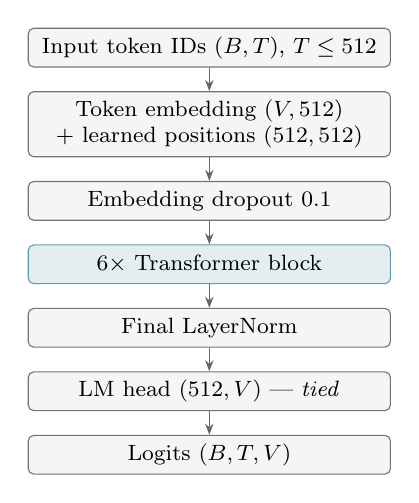
\begin{tikzpicture}[node distance=3mm, every node/.style={font=\footnotesize}]
\node[stage, minimum width=46mm] (ids) {Input token IDs $(B,T)$, $T \le 512$};
\node[stage, below=of ids, minimum width=46mm] (emb) {Token embedding $(V,512)$\\$+$ learned positions $(512,512)$};
\node[stage, below=of emb, minimum width=46mm] (drop) {Embedding dropout 0.1};
\node[hstage, below=of drop, minimum width=46mm] (blk) {$6\times$ Transformer block};
\node[stage, below=of blk, minimum width=46mm] (ln) {Final LayerNorm};
\node[stage, below=of ln, minimum width=46mm] (head) {LM head $(512,V)$ --- \emph{tied}};
\node[stage, below=of head, minimum width=46mm] (log) {Logits $(B,T,V)$};
\foreach \a/\b in {ids/emb, emb/drop, drop/blk, blk/ln, ln/head, head/log}
  \draw[flow] (\a) -- (\b);
\end{tikzpicture}
\end{minipage}\hfill
\begin{minipage}[c]{0.46\textwidth}
\centering
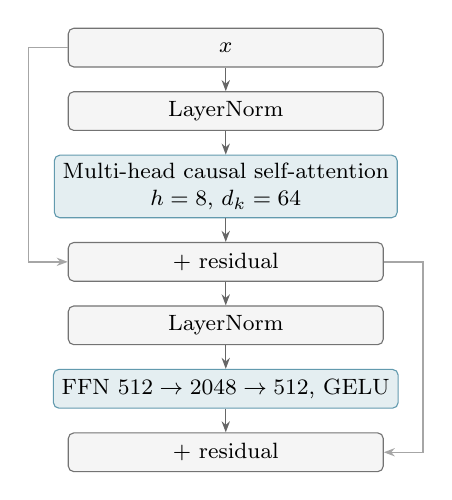
\begin{tikzpicture}[node distance=3mm, every node/.style={font=\footnotesize}]
\node[stage, minimum width=40mm] (x) {$x$};
\node[stage, below=of x, minimum width=40mm] (n1) {LayerNorm};
\node[hstage, below=of n1, minimum width=40mm] (at) {Multi-head causal self-attention\\$h=8$, $d_k=64$};
\node[stage, below=of at, minimum width=40mm] (a1) {$+$ residual};
\node[stage, below=of a1, minimum width=40mm] (n2) {LayerNorm};
\node[hstage, below=of n2, minimum width=40mm] (ff) {FFN $512 \to 2048 \to 512$, GELU};
\node[stage, below=of ff, minimum width=40mm] (a2) {$+$ residual};
\foreach \a/\b in {x/n1, n1/at, at/a1, a1/n2, n2/ff, ff/a2} \draw[flow] (\a) -- (\b);
\draw[flow, draw=black!35] (x.west) -- ++(-5mm,0) |- (a1.west);
\draw[flow, draw=black!35] (a1.east) -- ++(5mm,0) |- (a2.east);
\end{tikzpicture}
\end{minipage}
\caption{Left: the forward pass. Right: one pre-norm block expanded, with the
two residual paths drawn in grey. $V = 8{,}000$ for Model~H and $10{,}000$ for
Model~L; everything else is identical between the two models.}
\end{figure}

Classes: \texttt{GPT}, \texttt{TransformerBlock},
\texttt{MultiHeadCausalSelfAttention}, \texttt{FeedForward} and
\texttt{LayerNorm}, all in \texttt{hindi/model/transformer.py} and the mirrored
\texttt{nepali/model/transformer.py}.

\subsection{Why decoder-only?}

\begin{shortans}
The task is causal language modelling --- predict the next token given
everything before it. A decoder-only stack with causal masking is exactly that.
An encoder would let every position see every other position, which makes
next-token prediction trivial and useless.
\end{shortans}

\begin{notebox}[Common follow-up]
\textit{``Why not encoder-decoder?''} --- That architecture maps one sequence to
another, for translation or summarisation. I have one sequence and one
objective.
\end{notebox}

\section{Attention}

\begin{notebox}[Think of it like this]
It is a lookup in a library. Each token writes a \textbf{query} (``what am I
looking for?''), every token also advertises a \textbf{key} (``what am I
about?'') and carries a \textbf{value} (``here is my actual content''). You
match your query against all keys to get relevance scores, turn those into
weights, and take a weighted blend of the values.
\end{notebox}

\[
\mathrm{Attention}(Q,K,V) \;=\;
\mathrm{softmax}\!\left(\frac{QK^{\top}}{\sqrt{d_k}} + M\right) V
\]

\begin{center}\small
\begin{tabular}{llp{5.4cm}}
\toprule
\textbf{Symbol} & \textbf{Shape in my model} & \textbf{Meaning} \\
\midrule
$X$ & $(B, T, 512)$ & input to the block \\
$Q = XW_Q$ & $(B, 8, T, 64)$ & queries \\
$K = XW_K$ & $(B, 8, T, 64)$ & keys \\
$V = XW_V$ & $(B, 8, T, 64)$ & values \\
$QK^{\top}$ & $(B, 8, T, T)$ & raw relevance scores \\
$d_k$ & $64$ & per-head dimension \\
$M$ & $(1, 1, T, T)$ & additive causal mask \\
output & $(B, T, 512)$ & after $\times V$, concat, $W_O$ \\
\bottomrule
\end{tabular}
\end{center}

\textbf{The reshape, in words:} each projection produces $(B,T,512)$. A
\texttt{view} turns it into $(B,T,8,64)$ and a \texttt{transpose} into
$(B,8,T,64)$ --- eight independent 64-dimensional heads. After attention,
transpose and reshape back to $(B,T,512)$ and apply $W_O$.

\begin{figure}[htbp]
\centering
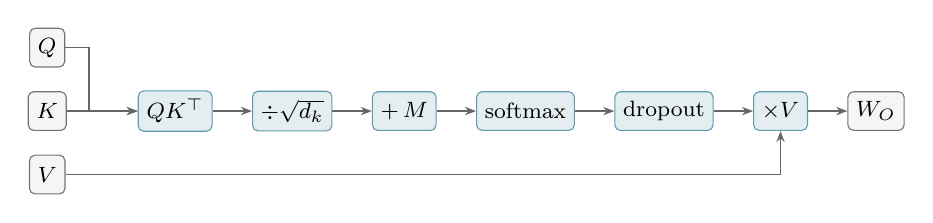
\begin{tikzpicture}[node distance=5mm, every node/.style={font=\footnotesize}]
\node[stage] (q) {$Q$};
\node[stage, below=3mm of q] (k) {$K$};
\node[stage, below=3mm of k] (v) {$V$};
\node[hstage, right=9mm of k] (s) {$QK^{\top}$};
\node[hstage, right=of s] (sc) {$\div\sqrt{d_k}$};
\node[hstage, right=of sc] (m) {$+\,M$};
\node[hstage, right=of m] (sm) {softmax};
\node[hstage, right=of sm] (dp) {dropout};
\node[hstage, right=of dp] (mv) {$\times V$};
\node[stage, right=of mv] (o) {$W_O$};
\draw[flow] (q.east) -- ++(3mm,0) |- (s.west);
\draw[flow] (k.east) -- (s.west);
\foreach \a/\b in {s/sc, sc/m, m/sm, sm/dp, dp/mv, mv/o} \draw[flow] (\a) -- (\b);
\draw[flow] (v.east) -- ++(3mm,0) -| (mv.south);
\end{tikzpicture}
\caption{The computation, end to end. $W_Q$, $W_K$ and $W_V$ are kept as three
separate \texttt{nn.Linear} layers rather than one fused matrix --- marginally
slower, but the three roles stay visible in the code.}
\end{figure}

\subsection{Why divide by \texorpdfstring{$\sqrt{d_k}$}{sqrt(d k)}?}

\begin{shortans}
Dot products of longer vectors grow in magnitude. With $d_k = 64$, if the
components are roughly independent with unit variance, the dot product has
variance about 64 and standard deviation about 8. Feeding numbers that large
into softmax saturates it, and the gradient through a saturated softmax is
almost zero. Dividing by $\sqrt{64} = 8$ brings the variance back to about 1.
\end{shortans}

\begin{vexample}[What saturation looks like]
\[
\mathrm{softmax}([2,1,0]) \approx [0.67,\,0.24,\,0.09] \quad\text{(informative)}
\]
\[
\mathrm{softmax}([16,8,0]) \approx [0.9997,\,0.0003,\,{\approx}0] \quad\text{(saturated, gradient} \approx 0)
\]
\end{vexample}

\begin{keypoint}
Without the scaling the model does not fail loudly --- it just trains badly,
because gradients through attention vanish.
\end{keypoint}

\section{Causal masking}

\begin{notebox}[Simple statement]
The model must not be allowed to look at the answer while predicting it.
\end{notebox}

For the sequence $A\,B\,C\,D$, the allowed pattern is lower triangular:

\begin{center}\small
\begin{tabular}{l|cccc}
& \textbf{key }$A$ & \textbf{key }$B$ & \textbf{key }$C$ & \textbf{key }$D$ \\
\midrule
query $A$ & yes & --- & --- & --- \\
query $B$ & yes & yes & --- & --- \\
query $C$ & yes & yes & yes & --- \\
query $D$ & yes & yes & yes & yes \\
\end{tabular}
\end{center}

and \textbf{not} every row full. When predicting what follows $C$, the model may
use $A$, $B$ and $C$, but not $D$ --- $D$ is the thing being predicted.

\begin{deeper}
\textbf{How it is implemented:} an upper-triangular mask built with
\texttt{torch.triu(..., diagonal=1)}, registered as a non-persistent buffer,
applied with \texttt{masked\_fill} with $-\infty$ \textbf{before} the softmax.

\medskip
\textbf{Why before softmax, and why $-\infty$?} Because softmax exponentiates:
$e^{-\infty} = 0$ exactly, and softmax then renormalises over the remaining
positions so the row still sums to 1. If you masked \emph{after} softmax you
would have to renormalise yourself, and the masked probability mass would
already have been mixed in.

\medskip
\textbf{Why exactly zero and not just small?} $\mathrm{softmax}(-\infty)$ is
exactly 0, and $0 \times v = 0$. There is no leakage at all, not even at
floating-point precision.
\end{deeper}

\begin{tcolorbox}[colback=conceptgreen!6,colframe=conceptgreen,
  title={\textbf{How my test verifies it}}]
\texttt{test\_causal\_mask\_blocks\_the\_future()} in
\texttt{hindi/tests/test\_model.py}:
\begin{enumerate}
\item Run the model, record the logits.
\item Perturb \textbf{every} token after position $t$.
\item Re-run and measure the largest change in the logits at positions $\le t$.
\item Result: \textbf{exactly 0.000e+00}.
\item The test also asserts the \textbf{converse} --- that outputs at the
perturbed positions \emph{do} change.
\end{enumerate}
\textbf{Why step 5 matters:} without it, a model that ignored its input entirely
would also pass. Checking only that nothing leaks is a one-sided test. Both
language suites pass 9/9.
\end{tcolorbox}

\section{The rest of the block}

\subsection{Pre-norm versus post-norm}

\begin{shortans}
I used pre-norm --- LayerNorm is applied to the input of each sublayer, before
attention and before the feed-forward network, rather than after the residual
addition.
\end{shortans}

\begin{deeper}
With pre-norm the residual path is a clean identity from input to output, so
gradients reach early layers without passing through a normalisation at every
step. Post-norm needs careful warmup to stay stable in deep stacks. At 6 layers
either would probably work; pre-norm is the safer default and is what modern
GPT-style models use.
\end{deeper}

\subsection{Feed-forward network and GELU}

\begin{shortans}
Two linear layers, $512 \to 2048 \to 512$, with GELU in between. The inner
dimension is $4\times$ the model dimension, the standard ratio.
\end{shortans}

\begin{deeper}
\textbf{Why have an FFN at all?} Attention mixes information \emph{across
positions} but is linear in the values. The FFN is where per-position
non-linear transformation happens. Without it, stacking attention layers would
collapse toward a linear operation.

\medskip
\textbf{Why GELU over ReLU?} It is smooth, so it has a non-zero gradient for
small negative inputs instead of ReLU's hard zero, and it is the standard
choice in GPT-style models.
\end{deeper}

\subsection{Residual connections}

\begin{shortans}
Each sublayer computes $x + \mathrm{sublayer}(\mathrm{norm}(x))$. The addition
gives gradients a direct path back through the network.
\end{shortans}

\begin{deeper}
Without them, gradients propagate through every transformation in series and in
a 6-layer stack shrink enough that early layers barely learn. Residuals also
let a block learn an \emph{adjustment} to its input rather than having to
reproduce the whole representation.
\end{deeper}

\section{Parameter count --- derive this live}

Configuration: $V = 8{,}000$ (H) or $10{,}000$ (L), $d = 512$, $n_{\text{layer}}
= 6$, $n_{\text{head}} = 8$, $d_{ff} = 2048$, block $= 512$, bias on, weight
tying on.

\begin{center}\small
\begin{tabular}{llrr}
\toprule
\textbf{Component} & \textbf{Formula} & \textbf{Model H} & \textbf{Model L} \\
\midrule
Token embedding & $V \times 512$ & 4,096,000 & 5,120,000 \\
Positional embedding & $512 \times 512$ & 262,144 & 262,144 \\
\textit{embedding subtotal} & & \textit{4,358,144} & \textit{5,382,144} \\
\midrule
Attention, per block & $4 \times (512^2 + 512)$ & 1,050,624 & 1,050,624 \\
FFN, per block & $(512{\cdot}2048{+}2048) + (2048{\cdot}512{+}512)$ & 2,099,712 & 2,099,712 \\
LayerNorms, per block & $2 \times (512 + 512)$ & 2,048 & 2,048 \\
\textit{block total} & & \textit{3,152,384} & \textit{3,152,384} \\
\midrule
6 blocks & $6 \times 3{,}152{,}384$ & 18,914,304 & 18,914,304 \\
Final LayerNorm & $512 + 512$ & 1,024 & 1,024 \\
\textbf{Non-embedding} & & \textbf{18,915,328} & \textbf{18,915,328} \\
\midrule
LM head & tied to token embedding & 0 & 0 \\
\textbf{Total} & & \textbf{23,273,472} & \textbf{24,297,472} \\
\bottomrule
\end{tabular}
\end{center}

\begin{keypoint}
The non-embedding count is \textbf{identical at 18,915,328 for both models},
and that is deliberate --- it means nobody can explain a difference in results
by saying one model was bigger. The only difference is the embedding table,
because the vocabularies differ.
\end{keypoint}

\begin{notebox}[This is also a test]
\texttt{test\_parameter\_count\_matches\_analytic\_estimate()} asserts the
analytic formula against the loaded model, and \texttt{GPT.parameter\_count()}
returns the breakdown.
\end{notebox}

\subsection{Weight tying}

\begin{shortans}
The output projection shares its matrix with the input token embedding. For
Model~H that saves $8{,}000 \times 512 = \textbf{4,096,000}$ parameters, roughly
15\% of the model.
\end{shortans}

\begin{deeper}
Both matrices relate the same vocabulary to the same 512-dimensional space ---
one maps ID $\rightarrow$ vector, the other vector $\rightarrow$ score per ID.
Two independent representations of the same vocabulary are redundant at this
scale, and tying also acts as a regulariser.

\medskip
\textit{Downside?} It constrains input and output representations to live in
the same space, which at very large scale can cost a little quality. At 23M
parameters against a 25M budget, spending 4M on a second copy of the vocabulary
was clearly the worse trade. \texttt{test\_weight\_tying\_shares\_storage()}
checks they are the same storage, not merely equal values.
\end{deeper}

\subsection{Positional embeddings}

\begin{shortans}
Learned absolute positional embeddings --- a $(512, 512)$ table added to the
token embeddings.
\end{shortans}

\begin{deeper}
\textbf{Why positions at all?} Self-attention is permutation invariant: shuffle
the input tokens and, without position information, the attention output set is
unchanged. ``Ram beat Shyam'' and ``Shyam beat Ram'' would be identical to the
model.

\medskip
\textbf{Why learned rather than sinusoidal?} The model is trained and evaluated
at one fixed context length, so the extrapolation advantage of sinusoidal
encodings does not apply, and learned positions let the model allocate
resolution where the data actually needs it.

\medskip
\textbf{What it costs:} 512 is a hard ceiling --- there is no embedding row for
position 512, so the model cannot run on a longer sequence without retraining
the table.
\texttt{test\_sequence\_longer\_than\_block\_size\_is\_rejected()} asserts this
fails loudly rather than silently misbehaving. Both alternatives are
implemented: \texttt{sinusoidal\_positional\_encoding()} exists, and
\texttt{pos\_encoding: none} is what the bonus ablation uses.
\end{deeper}

\section{Training}

\begin{center}\small
\begin{tabular}{ll}
\toprule
Optimiser & AdamW, $\beta = (0.9,\,0.95)$ \\
Weight decay & 0.1, applied only where \texttt{param.dim() >= 2} \\
Peak / min learning rate & $6\times10^{-4}$ $\rightarrow$ $6\times10^{-5}$ \\
Schedule & 500 warmup steps, then cosine (\texttt{CosineWarmupSchedule}) \\
Gradient clipping & 1.0, applied \textbf{after} \texttt{unscale\_} \\
Micro-batch $\times$ accumulation & $32 \times 2 \times 512 = $ \textbf{32,768 tokens per step} \\
Precision & bfloat16 \\
Seed & 20260902 \\
Planned steps & 15,000 \\
Steps reached & H 14,520 / L 14,440 (11-hour wall-clock guard) \\
Tokens consumed & H 475,791,360 / L 473,169,920 \\
Hardware & Kaggle Tesla T4, 10.99 h each, ${\approx}12{,}024$ / $11{,}958$ tok\,s$^{-1}$ \\
\bottomrule
\end{tabular}
\end{center}

\begin{deeper}[Why each of those choices]
\textbf{AdamW rather than Adam:} it decouples weight decay from the gradient
update. In plain Adam, L2 regularisation gets scaled by the adaptive learning
rate and is therefore applied inconsistently across parameters.

\smallskip
\textbf{$\beta_2 = 0.95$ rather than 0.999:} a shorter second-moment window
adapts faster, the common choice for LM pretraining at this scale.

\smallskip
\textbf{Decay only matrices:} LayerNorm gains and biases are not weights in the
same sense --- decaying them just shrinks them toward zero for no regularisation
benefit. The filter is \texttt{param.dim() >= 2} in
\texttt{configure\_optimizers()}.

\smallskip
\textbf{Warmup:} at step 0 Adam's moment estimates are unreliable and the
parameters are random, so a full-size step can push the model somewhere it
takes a long time to recover from.

\smallskip
\textbf{Cosine decay:} a large learning rate early explores, a small one late
refines, and cosine is smooth without a hand-tuned staircase.

\smallskip
\textbf{Gradient accumulation:} the 32,768-token effective batch does not fit in
T4 memory as one micro-batch. Accumulating 2 micro-batches of 32 decouples the
statistical batch size from the memory limit. On a smaller GPU you lower
\texttt{batch\_size} and raise \texttt{grad\_accum\_steps} to keep the product
constant.

\smallskip
\textbf{Clip after unscale:} with mixed precision the loss is scaled up to avoid
underflow, so gradients are scaled too. Clipping before unscaling would clip
the \emph{scaled} gradients and the effective threshold would depend on the
scale factor.
\end{deeper}

\subsection{Checkpointing and resume}

\begin{figure}[htbp]
\centering
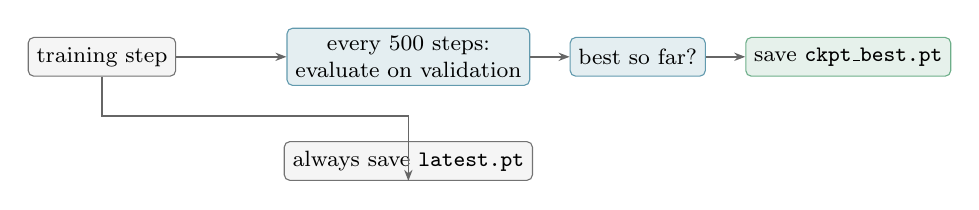
\begin{tikzpicture}[node distance=5mm, every node/.style={font=\footnotesize}]
\node[stage] (t) {training step};
\node[hstage, right=14mm of t] (ev) {every 500 steps:\\evaluate on validation};
\node[hstage, right=of ev] (best) {best so far?};
\node[gstage, right=of best] (ck) {save \texttt{ckpt\_best.pt}};
\node[stage, below=7mm of ev] (lat) {always save \texttt{latest.pt}};
\draw[flow] (t) -- (ev);
\draw[flow] (ev) -- (best);
\draw[flow] (best) -- (ck);
\draw[flow] (t.south) -- ++(0,-5mm) -| (lat.south);
\end{tikzpicture}
\caption{Checkpointing. The payload from \texttt{\_checkpoint\_payload()} is
model weights, optimizer state, scheduler state, training step, best validation
loss, tokens seen, both RNG states and the full config.}
\end{figure}

\begin{deeper}
\textbf{Why all of it?} Restoring only the weights restarts the optimiser's
moment estimates and the learning-rate schedule from scratch, which is a
different training run. Restoring the RNG states means the data order continues
rather than restarting.

\medskip
\textbf{Evidence it works:} I verified resume across three deliberately killed
sessions before starting the real runs, because the whole thing runs on Kaggle
and sessions do die.

\medskip
\textbf{Why the 11-hour guard?} So a dying session could never leave an unusable
state. It fired at steps 14,520 and 14,440 of a planned 15,000 --- costing about
3\% of the token budget.
\end{deeper}

\section{Intrinsic results}

\begin{center}\small
\begin{tabular}{lrr}
\toprule
& \textbf{Model H} & \textbf{Model L} \\
\midrule
Test cross-entropy (nats) & 3.3109 & 3.8433 \\
\textbf{Test perplexity} & \textbf{27.41} & 46.68 \\
Bits per token & 4.7766 & 5.5447 \\
Bytes per token & 8.875 & 11.441 \\
\textbf{Test bits-per-byte} & 0.5382 & \textbf{0.4846} \\
Tokens scored & 1,999,872 & 1,999,872 \\
Bytes scored & 17,749,798 & 22,880,653 \\
Best validation loss / ppl & 3.3402 / 28.22 @ 14,500 & 3.5953 / 36.43 @ 14,000 \\
\bottomrule
\end{tabular}
\end{center}

The full perplexity-versus-bits-per-byte argument is Chapter~8 --- that is the
single most important section in this guide.

\section{Generation}

Setup: 64 held-out prefixes of 64 tokens each, continued for 64 tokens, scored
against the true continuations.

\begin{center}\small
\begin{tabular}{llrrrrrr}
\toprule
\textbf{Model} & \textbf{Decoding} & \textbf{BLEU-4} & \textbf{chrF++} & \textbf{ROUGE-L} & \textbf{Repetition} & \textbf{Distinct-1} & \textbf{Distinct-2} \\
\midrule
H & greedy & 1.96 & 12.49 & 0.093 & 0.598 & 0.172 & 0.313 \\
H & $T=0.5$ & 1.80 & 14.33 & 0.096 & 0.212 & 0.275 & 0.602 \\
H & $T=1.0$ & 1.01 & \textbf{16.29} & \textbf{0.100} & 0.002 & 0.520 & 0.939 \\
H & $T=1.5$ & 0.16 & 14.67 & 0.053 & 0.000 & 0.702 & 0.992 \\
\midrule
L & greedy & 2.37 & 14.48 & 0.081 & 0.577 & 0.179 & 0.263 \\
L & $T=0.5$ & 1.88 & 16.54 & \textbf{0.092} & 0.190 & 0.345 & 0.611 \\
L & $T=1.0$ & 1.69 & \textbf{18.05} & 0.079 & 0.001 & 0.634 & 0.948 \\
L & $T=1.5$ & 0.78 & 16.13 & 0.035 & 0.000 & 0.793 & 0.995 \\
\bottomrule
\end{tabular}
\end{center}

\begin{vexample}[Temperature, with numbers]
Temperature divides the logits before softmax. Starting from $A = 0.7$,
$B = 0.2$, $C = 0.1$:
\begin{itemize}
\item $T < 1$ (say 0.5) \textbf{sharpens}: the gap widens, $A$ moves toward 1.
More confident, more repetitive.
\item $T = 1$ leaves the distribution unchanged.
\item $T > 1$ (say 1.5) \textbf{flattens}: the three move toward equal. More
diverse, more errors.
\item $T \to 0$ is greedy decoding --- always take the argmax.
\end{itemize}
\end{vexample}

\begin{deeper}
\textbf{Why greedy degenerates.} At greedy, 58--60\% of generated 4-grams are
repeats. That is not a bug in the model --- it follows from the rule. Greedy
always takes the argmax, so the moment the model re-enters a state it has been
in, it produces the same continuation, with no mechanism to escape the loop.

\medskip
\textbf{The clean finding.} $T = 1.0$ gives the best chrF++ for both models
\emph{and} kills repetition. The usual quality--diversity trade-off does not
bind anywhere in this range.
\end{deeper}

\begin{shortans}
BLEU counts exact 4-gram overlap with a reference, and an open-ended
continuation has no particular reason to reproduce the one true continuation's
4-grams --- a perfectly fluent continuation can score near zero. chrF++ is the
metric I would defend here, because it works on character $n$-grams: in
morphologically rich Devanagari, changing one suffix destroys a whole-word
match but leaves most character $n$-grams intact. ROUGE-L is computed over
whitespace tokens, which under-segment Devanagari, making it the least reliable
of the three. I report all three because the specification requires them, and I
say which one I trust.
\end{shortans}

\section{Attention analysis}

\textbf{Attention entropy} measures how spread out a head's attention is:
$H = -\sum p \log p$. Low entropy means one key takes almost all the weight
(sharp, focused); high entropy means the weight is spread evenly (diffuse).

\textbf{Mean attention distance} measures how far back a head looks, on average,
from a query position to the key positions it attends to. Small = local,
large = long-range.

\begin{center}\small
\begin{tabular}{lrr}
\toprule
& \textbf{Model H} & \textbf{Model L} \\
\midrule
Mean entropy (nats) & 3.2047 & 3.0898 \\
Uniform baseline & 5.2565 & 5.2565 \\
Mean distance (tokens) & 62.36 & 54.51 \\
Local-head fraction & 0.0625 & 0.1250 \\
\bottomrule
\end{tabular}
\end{center}

\begin{keypoint}
\textbf{Why compute the uniform baseline?} Because ``entropy 3.2'' means nothing
on its own. Against a uniform baseline of 5.2565 you can say the heads are
meaningfully more focused than chance. Without it the number is
uninterpretable. (\texttt{uniform\_baseline\_entropy()} in
\texttt{hindi/eval/attention.py}.)
\end{keypoint}

\begin{center}\small
\begin{tabular}{lll}
\toprule
\textbf{Layer} & \textbf{Model H (entropy @ distance)} & \textbf{Model L} \\
\midrule
0 & 4.16 @ 45.8 & 3.90 @ 36.0 \\
1 & 3.09 @ 21.9 & 3.17 @ 17.1 \\
2 & 1.49 @ \;7.6 & 1.81 @ 10.6 \\
\textbf{3} & \textbf{0.06 @ \;1.3} & \textbf{0.14 @ \;1.1} \\
4 & 1.49 @ 22.4 & 1.32 @ \;5.6 \\
5 & 2.99 @ 151.4 & 2.48 @ 81.3 \\
\bottomrule
\end{tabular}
\end{center}

\begin{shortans}
Both models independently grew a \textbf{previous-token head at layer 3} ---
entropy 0.06 at distance 1.3 for Hindi, 0.14 at distance 1.1 for Nepali.
Different languages, different tokenizers, different random seeds, same
structure. Attention is diffuse at layer 0, sharpens to layer 3, then broadens
again at layer 5.
\end{shortans}

\begin{deeper}
\textbf{Why would a previous-token head emerge?} Language is locally
predictable --- the immediately preceding token is the single most informative
context for the next one, especially for morphology and agreement. A head that
copies ``what came immediately before'' is cheap to learn and immediately
useful, so gradient descent finds it early.
\end{deeper}

\begin{trap}[Say this before they ask]
``This is a consistent pattern, not evidence of a functional role. I measured
which heads are sharp and how far they look. I did \textbf{not} establish what
any head contributes to the prediction --- that would need ablating a head and
re-scoring, which I did not run.''
\end{trap}

% =======================================================================
\chapter{Phase 3 --- Reasoning Finetuning}
\chaptermark{Phase 3 --- Reasoning Finetuning}
% =======================================================================

\section{Why synthetic data?}

\begin{shortans}
So that I know the ground-truth answer by construction and can control the
train/test relationship exactly. The brief also requires it --- the primary
finetuning set must not be a downloaded benchmark.
\end{shortans}

\begin{deeper}
With a generator I can guarantee that test questions use entity names and
sentence templates the model has never seen, and \emph{assert} it. With a
downloaded dataset I would have no idea what overlaps what.
\end{deeper}

\section{The four task families}

All examples below are real rows from
\texttt{hindi/reasoning/data/test.jsonl} and
\texttt{nepali/reasoning/data/test.jsonl}.

\begin{vexample}[\texttt{compare2} --- one-step comparison, 2 candidates]
\dn{ध्यान दीजिए: प्रवीण वरुण से हल्का है। भारी कौन है?} $\rightarrow$
\textbf{\dn{वरुण}}

\smallskip
\textit{(Praveen is lighter than Varun. Who is heavier?)} --- note the direction
flip: ``lighter'' in the premise, ``heavier'' in the question.
\end{vexample}

\begin{vexample}[\texttt{numeric2} --- explicit quantities, 2 candidates]
\dn{दिया गया है कि चंदा का वज़न ६७ किलो है और मालती का वज़न ४८ किलो है। हल्की कौन है?}
$\rightarrow$ \textbf{\dn{मालती}}
\end{vexample}

\begin{vexample}[\texttt{numeric3} --- explicit quantities, 3 candidates]
\dn{यहाँ प्रवीण की उम्र ५९ साल, नवीन की उम्र ६७ साल, तथा अरुण की उम्र २४ साल है। सबसे बड़ा कौन है?}
$\rightarrow$ \textbf{\dn{नवीन}}
\end{vexample}

\begin{vexample}[\texttt{transitive3} --- two-hop chain, 3 candidates]
\dn{शारदा सविता से भारी है। इसी तरह सविता मालती से भारी है। सबसे भारी कौन है?}
$\rightarrow$ \textbf{\dn{शारदा}}

\smallskip
\textit{(Sharda $>$ Savita, Savita $>$ Malti. Who is heaviest?)}
\end{vexample}

\begin{vexample}[Nepali --- note the Arabic digits]
\dn{दिइएको छ कि रबिनको उमेर 22 वर्ष र भोजराजको उमेर 49 वर्ष छ। जेठो को हो?}
$\rightarrow$ \textbf{\dn{भोजराज}}

\smallskip
Hindi uses Devanagari digits (\dn{५९}, \dn{६७}); Nepali uses Arabic digits.
That asymmetry is the byte-fallback fix described in Chapter~3.
\end{vexample}

\subsection{Why \texttt{transitive3} is the real test}

\begin{center}
\begin{tabular}{rcl}
Premise 1: & $A > B$ & \\
Premise 2: & & $B > C$ \\
\midrule
Question: & \multicolumn{2}{l}{who is largest? \qquad Answer: $A$} \\
\end{tabular}
\end{center}

\begin{deeper}
\textbf{What information is needed?} You must chain the two inequalities ---
neither premise alone identifies $A$ as the maximum.

\smallskip
\textbf{Why is this transitive reasoning?} It requires the inference
$A > B \wedge B > C \Longrightarrow A > C$, which is stated nowhere in the
prompt.

\smallskip
\textbf{What would a shortcut-based model do?} Notice that \textbf{$B$ is the
only name mentioned twice} and pick it on salience. That is exactly what my
models do --- see Section~5.6.
\end{deeper}

\section{Dataset construction and leakage control}

\begin{figure}[htbp]
\centering
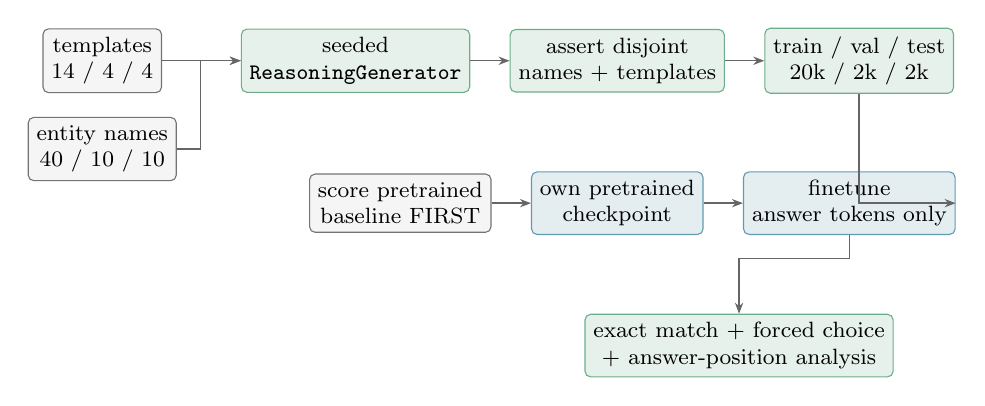
\begin{tikzpicture}[node distance=5mm, every node/.style={font=\footnotesize}]
\node[stage] (t) {templates\\14 / 4 / 4};
\node[stage, below=3mm of t] (n) {entity names\\40 / 10 / 10};
\node[gstage, right=10mm of t] (g) {seeded\\\texttt{ReasoningGenerator}};
\node[gstage, right=of g] (a) {assert disjoint\\names + templates};
\node[gstage, right=of a] (s) {train / val / test\\20k / 2k / 2k};
\node[hstage, below=10mm of a] (ck) {own pretrained\\checkpoint};
\node[hstage, right=of ck] (ft) {finetune\\answer tokens only};
\node[stage, left=of ck] (sc) {score pretrained\\baseline FIRST};
\node[gstage, below=10mm of ft, xshift=-14mm] (ev) {exact match $+$ forced choice\\$+$ answer-position analysis};
\draw[flow] (t) -- (g);
\draw[flow] (n.east) -- ++(3mm,0) |- (g.west);
\draw[flow] (g) -- (a);
\draw[flow] (a) -- (s);
\draw[flow] (s.south) |- (ft.east);
\draw[flow] (sc) -- (ck);
\draw[flow] (ck) -- (ft);
\draw[flow] (ft.south) -- ++(0,-3mm) -| (ev.north);
\end{tikzpicture}
\caption{Generation and finetuning. Scoring the pretrained baseline
\emph{before} finetuning is a sequencing constraint --- once the weights change
that number is unrecoverable without retraining.}
\end{figure}

\begin{shortans}
Leakage is controlled on two axes at once. The 40/10/10 entity names and the
14/4/4 sentence templates are both disjoint across splits, so a test question is
about people the model has never seen, phrased in a way it has never seen.
\end{shortans}

\begin{deeper}
Both properties are \textbf{asserted inside \texttt{main()} of
\texttt{generate.py}}, not assumed, and recorded in
\texttt{dataset\_stats.json} as
\texttt{entity\_names\_disjoint\_across\_splits: true} and
\texttt{templates\_disjoint\_across\_splits: true}. The Hindi and Nepali sets
share no sentence, no entity name and no template.

\medskip
\textit{``Why hold out both?''} Holding out only names would let the model pass
by memorising which template implies which answer position. Holding out only
templates would let it memorise per-name answer priors. You need both axes
closed.
\end{deeper}

\subsection{The gender-agreement leak}

\begin{trap}[A defect I found and fixed --- good to volunteer]
\textbf{Problem:} Hindi adjectives inflect for gender, so a question like ``who
is smallest?'' asked about one woman and two men has only one grammatically
well-formed answer --- solvable without comparing anything.

\smallskip
\textbf{Detection:} inspecting generated examples for shortcuts.
\textbf{181 of 400} sampled examples were solvable that way.

\smallskip
\textbf{Why:} the generator drew entity names independently of gender, and the
adjective had to agree with \emph{some} gender.

\smallskip
\textbf{Fix:} \texttt{inflect()} plus drawing all entities in an example from one
gender, so agreement carries no information about the answer.

\smallskip
\textbf{Lesson:} in an inflected language, grammar itself can be a leak channel.
\end{trap}

\section{Finetuning protocol}

\begin{center}\small
\begin{tabular}{ll}
\toprule
Starting point & each model's \textbf{own} Phase 2 checkpoint \\
Tokenizer & held fixed from Phase 1 \\
Loss & answer tokens only (\texttt{ignore\_index=-1} over the prompt) \\
Batching & grouped by length, \textbf{not} padded \\
Epochs / batch & 2 / 32 \\
Peak / min LR & $6\times10^{-5}$ / $6\times10^{-6}$ \\
Warmup & 100 steps \\
Evaluation interval & every \textbf{20} steps \\
Seed & 20260914 \\
Precision & float16 with a \texttt{GradScaler} \\
\bottomrule
\end{tabular}
\end{center}

\begin{deeper}[Why each choice]
\textbf{Answer-token-only loss:} if loss covered the whole sequence, most of it
would be question text and the model would be rewarded for memorising phrasing
rather than producing the right answer. Masking the prompt means the gradient
only ever comes from the answer.

\smallskip
\textbf{Length-grouped batches --- necessary, not cosmetic:} with learned
absolute positional embeddings, left padding would shift the position index of
every real token. The same content would sit at position 3 in one batch and 7
in another, and the model would see a different positional embedding for it.
Grouping by length avoids padding entirely.

\smallskip
\textbf{Learning rate one tenth of pretraining:} the model already holds a
language model worth keeping. A pretraining-sized step overwrites it before the
task is learned; the usual failure mode is a model that answers in the right
format but has forgotten how to read the question.

\smallskip
\textbf{float16 rather than bfloat16:} the Kaggle T4 is compute capability 7.5
and has no bfloat16 support, so the pretraining config could not be reused.
float16 needs a \texttt{GradScaler} to avoid gradient underflow.
\end{deeper}

\begin{notebox}[A guard worth mentioning]
The finetuning script \textbf{asserts} that the tokenizer vocabulary size
matches the checkpoint, rather than trusting the config file. That mismatch is
exactly the kind you do not notice until the results are garbage.
\end{notebox}

\section{Exact match versus forced choice}

\begin{center}\small
\begin{tabular}{p{6.4cm}p{6.4cm}}
\toprule
\textbf{Exact match} & \textbf{Forced choice} \\
\midrule
Greedy-decode an answer. Does the string equal the gold answer? &
Take only the entity names the question actually contains. Score each one's
length-normalised mean log-probability. Does the highest-scoring one match? \\[4pt]
Honest end-to-end measure --- but pinned at 0 before finetuning, so it cannot
separate ``learned nothing'' from ``knows it but cannot phrase it''. &
Removes the formatting problem entirely. Chance rate computed per example from
the number of candidates. \\
\bottomrule
\end{tabular}
\end{center}

\begin{keypoint}
\textbf{The chance rate.} \texttt{compare2} and \texttt{numeric2} have 2
candidates (chance 50\%); \texttt{numeric3} and \texttt{transitive3} have 3
(chance 33.3\%). Averaged over the equal-sized families:
$(0.5 + 0.5 + \tfrac13 + \tfrac13)/4 = \mathbf{0.4167}$. It is computed per
example from the actual candidate count, not assumed.
\end{keypoint}

\begin{center}\small
\begin{tabular}{lrrrr}
\toprule
& \textbf{H pretrained} & \textbf{H finetuned} & \textbf{L pretrained} & \textbf{L finetuned} \\
\midrule
Exact match & 0.00\% & \textbf{35.15\%} & 0.00\% & \textbf{29.45\%} \\
Forced choice & 39.80\% & 36.35\% & 38.80\% & 39.30\% \\
Chance rate & 41.67\% & 41.67\% & 41.67\% & 41.67\% \\
Answer-token loss & 5.2439 & 0.9408 & 5.5367 & 1.4351 \\
Answer-token perplexity & 189.40 & 2.56 & 253.84 & 4.20 \\
\bottomrule
\end{tabular}
\end{center}

\begin{sayit}[The answer to give --- observation, interpretation, limit]
\textbf{Observation:} exact match rose from zero to 35.15\% and 29.45\%, and
answer-token loss fell by more than four nats in both models.

\smallskip
\textbf{Interpretation:} finetuning taught the models to emit a candidate name
in the expected position and format. The loss collapse is consistent with that
and with nothing stronger.

\smallskip
\textbf{What it does not show:} under forced choice both models sit at or below
the 41.67\% chance rate, and per task the scores land close to their individual
chance rates. The result does not establish that either model learned the
comparison operation.
\end{sayit}

\begin{center}\small
\begin{tabular}{lrrrrr}
\toprule
\textbf{Task} & \textbf{Chance} & \textbf{H exact} & \textbf{L exact} & \textbf{H forced} & \textbf{L forced} \\
\midrule
\texttt{compare2} & 50.0\% & 47.40\% & 40.20\% & 50.40\% & 49.40\% \\
\texttt{numeric2} & 50.0\% & 47.40\% & 38.00\% & 47.00\% & 51.80\% \\
\texttt{numeric3} & 33.3\% & 33.40\% & 26.20\% & 33.20\% & 32.40\% \\
\texttt{transitive3} & 33.3\% & 12.40\% & 13.40\% & \textbf{14.80\%} & \textbf{23.60\%} \\
\bottomrule
\end{tabular}
\end{center}

Three families sit on their chance line. The two-hop family falls
\textbf{below} it.

\section{Error analysis}

\begin{center}\small
\begin{tabular}{lrrrr}
\toprule
\texttt{transitive3}, finetuned & \textbf{answered $A$} & \textbf{answered $B$} & \textbf{answered $C$} & \textbf{off-prompt} \\
& (first) & (middle) & (last) & \\
\midrule
Gold distribution & 47.4\% & \textbf{0.0\%} & 52.6\% & --- \\
Model H & \textbf{0.0\%} & \textbf{72.6\%} & 25.4\% & 2.0\% \\
Model L & 3.2\% & 41.8\% & 26.2\% & 28.8\% \\
\bottomrule
\end{tabular}
\end{center}

\begin{sayit}[The argument, in one breath]
The chain is stated as $A$ rel $B$, $B$ rel $C$, so the extremes are always $A$
and $C$ and the middle entity is \textbf{never} correct. Model H nevertheless
picks the middle entity 72.6\% of the time and the first entity in
\textbf{none}. $B$ is the only name mentioned twice. So the model is selecting
on surface salience, not following the inequality --- and that is precisely why
this family scores \emph{below} chance, because uniform guessing would at least
hit $A$ and $C$ sometimes.
\end{sayit}

\textbf{One-hop recency bias}, Model H: on \texttt{compare2} it answers the
second-named entity 62.0\% of the time against a 48/52 gold split, and on
\texttt{numeric2} 65.0\% against a 50/50 split --- roughly two to one toward the
most recently mentioned name.

\begin{center}\small
\begin{tabular}{lrr}
\toprule
\textbf{Answers with a name not in the prompt} & \textbf{Model H} & \textbf{Model L} \\
\midrule
\texttt{compare2} & 7.2\% & 19.2\% \\
\texttt{numeric2} & 0.0\% & 25.0\% \\
\texttt{numeric3} & 1.0\% & 21.2\% \\
\texttt{transitive3} & 2.0\% & 28.8\% \\
\bottomrule
\end{tabular}
\end{center}

\begin{keypoint}
Model L emits memorised \emph{training} names (\dn{सिर्जना}, \dn{निरु}) instead
of a candidate in front of it. Before finetuning both models do this
essentially 100\% of the time. So the resource tier shows up not as reasoning
accuracy --- both are at chance there --- but as \textbf{groundedness}. The
better-pretrained model is better at \emph{using its input}, which is a weaker
and far more defensible claim than ``better reasoning''.
\end{keypoint}

\section{Overfitting and checkpoint selection}

\begin{shortans}
Validation loss bottoms out at \textbf{step 60} and rises afterwards while
training loss keeps falling to 0.4441 (H) and 0.6048 (L), reaching validation
3.5188 and 3.5911 by step 1,250. I save on best validation loss, so the
evaluated checkpoints are step 60 --- the overfitting visible in the curve never
reached my reported numbers.
\end{shortans}

\begin{deeper}
\textbf{Why did it happen?} With only 40 entity names and 14 templates,
memorising which answer tends to be right is easier than learning to read the
question. The training distribution is too narrow in two independent ways: too
few entities, and every example of a template is identical apart from slot
fillers, so the surface form carries almost no entropy.
\end{deeper}

\begin{trap}[The Run A / Run B story --- volunteer this]
My first finetuning run evaluated every \textbf{100} steps and selected its best
checkpoint at step 100 --- which is exactly where warmup ends and the learning
rate first reaches its peak --- with validation loss rising monotonically after
that. The grid was too coarse to locate the real optimum.

\smallskip
I moved to a \textbf{20}-step grid with nothing else changed, and Model L went
from 14.90\% to 29.45\% exact match, Model H from 32.70\% to 35.15\%. The
superseded run is kept in \texttt{report/phase3/run\_a\_40names/} rather than
deleted.

\smallskip
That is a one-variable change with a measured effect, and keeping the old run
is good practice.
\end{trap}

\section{Attention before and after finetuning}

Measured on the same held-out reasoning prompts, all of identical token length,
so that neither prompt content nor sequence length could masquerade as a
finetuning effect.

\begin{center}\small
\begin{tabular}{llrrl}
\toprule
\textbf{Model} & \textbf{Checkpoint} & \textbf{Mean entropy} & \textbf{Mean distance} & \textbf{Uniform baseline} \\
\midrule
H & pretrained (step 14,500) & 1.9102 & 10.303 & 2.9545 (length 46) \\
H & finetuned (step 60) & 1.8691 & 10.360 & \\
L & pretrained (step 14,000) & 1.8327 & \;9.415 & 2.8061 (length 39) \\
L & finetuned (step 60) & 1.7833 & 10.157 & \\
\bottomrule
\end{tabular}
\end{center}

\textbf{Observation:} attention became slightly sharper \emph{and} slightly
longer-range at the same time in both models, most visibly in Model L where
mean distance rises 0.74 positions on a 39-token prompt. The largest per-head
shifts concentrate in the middle layers --- where Phase 2 found the
previous-token heads.

\textbf{Interpretation:} consistent with a shift toward attending to the entity
names scattered across the prompt rather than to local context.

\begin{trap}[Limitation --- state it yourself]
``This identifies which heads changed, not what they compute. Showing that
these heads perform the comparison would require ablating a head and
re-scoring, which I did not run.''
\end{trap}

% =======================================================================
\chapter{Cross-Phase Questions}
\chaptermark{Cross-Phase Questions}
% =======================================================================

\begin{qabox}{How did tokenizer design affect Phase 2?}
Directly and decisively. Model L's BPE at 10,000 produces 11.44 bytes per token
against Model H's 8.88. That single property is large enough to reverse the
ranking between perplexity and bits-per-byte. Any cross-language perplexity
comparison in this project is a statement about tokenizers at least as much as
about models.
\end{qabox}

\begin{qabox}{How did Phase 1 data quality affect Phase 2?}
Model L's corpus is nominally larger (520M vs 485M train tokens) but 91.6\% of
its manual lane is a single news source, while Model H draws on five distinct
manual sources and five downloaded partitions. Model L saw \emph{more} tokens of
\emph{narrower} text. That is a plausible contributor to its higher perplexity
--- though I cannot cleanly separate it from tokenizer effects.
\end{qabox}

\begin{qabox}{Which Phase 1 decision most affected later phases?}
The missing byte fallback on the Nepali tokenizer. In Phase 1 it appeared only
as a column of zeros I misread as a good score. In Phase 2 it surfaced as a
0.17--0.34\% unknown-token rate. In Phase 3 it became outright corruption --- no
Devanagari digit in the vocabulary, so 4.8\% of the generated reasoning corpus
became \texttt{<unk>}. One configuration flag, invisible for two phases, then
responsible for a data defect.
\end{qabox}

\begin{qabox}{Why might a model with better language modelling still fail reasoning?}
Because next-token prediction and relational inference are different
capabilities. Both my models are at chance on the comparison itself despite
being usable language models. What better pretraining bought was groundedness
--- Model H answers from the given candidates 93--100\% of the time against
Model L's 71--81\% --- not reasoning.
\end{qabox}

\begin{qabox}{How did Phase 2 attention analysis help Phase 3?}
It gave me a baseline. Phase 2 located previous-token heads at layer 3; Phase 3
found the largest finetuning-induced shifts in those same middle layers.
Without the Phase 2 measurement, the Phase 3 deltas would have had nothing to
be relative to.
\end{qabox}

\begin{qabox}{What evidence supports your main conclusion, and what does not?}
\textbf{Supports:} that most of the H/L perplexity gap is tokenizer
granularity --- the bytes-per-token measurement (8.88 vs 11.44) is large enough
to flip the ordering, and the flip is exactly what bits-per-byte shows.

\smallskip
\textbf{Does not:} bits-per-byte is tokenizer-neutral but \textbf{not
corpus-neutral}. The two models are scored on different text of different
intrinsic difficulty, so I cannot conclude Model L is the better language model
--- only that the perplexity gap overstates the difference. Separating those
would need a parallel evaluation set, which I do not have.
\end{qabox}

\begin{qabox}{Strongest result? Weakest? Most surprising? What next?}
\textbf{Strongest:} the perplexity/bits-per-byte reversal --- clean,
mechanistically explained, derivable live.

\smallskip
\textbf{Weakest:} the reasoning results. Both models are at chance, and the
training distribution was too narrow to give finetuning a fair chance.

\smallskip
\textbf{Most surprising:} that both models independently grew a
near-deterministic previous-token head at layer 3, with different languages,
tokenizers and seeds.

\smallskip
\textbf{Next experiment:} head ablation --- disable the heads that moved most
during finetuning and re-score the reasoning test set. That converts the
attention analysis from correlational to causal, which is the main thing it
currently lacks.
\end{qabox}

% =======================================================================
\chapter{Code-Level Questions}
\chaptermark{Code-Level Questions}
% =======================================================================

\section{Where everything lives}

\begin{longtable}{@{}p{2.6cm}p{4.4cm}p{7.4cm}@{}}
\toprule
\textbf{Area} & \textbf{File} & \textbf{Key names} \\
\midrule
\endfirsthead
\toprule
\textbf{Area} & \textbf{File} & \textbf{Key names} \\
\midrule
\endhead
Cleaning & \texttt{scripts/clean\_lib.py} & \texttt{normalize\_text()}, \texttt{devanagari\_ratio()}, \texttt{malformed\_ratio()}, \texttt{is\_too\_short()}, \texttt{langdetect\_verdict()}, \texttt{dedup\_key()}, \texttt{strip\_latin\_tokens()} \\
Hindi pipeline & \texttt{hindi/data/pipeline/} & \texttt{download\_hindi.py}, \texttt{ingest\_manual.py}, \texttt{ingest\_wikipedia\_dump.py}, \texttt{clean\_hindi.py}, \texttt{split\_hindi.py} \\
Nepali pipeline & \texttt{nepali/scripts/} & \texttt{s00\_doctor.py} \ldots{} \texttt{s14\_corpus\_stats.py}, \texttt{run\_pipeline.py} \\
Nepali dedup & \texttt{corpuslib/dedup.py} & \texttt{MinHasher}, \texttt{shingles()}, \texttt{build\_lsh\_buckets()}, \texttt{remove\_near\_duplicates()}, \texttt{find\_contaminated()} \\
Nepali language ID & \texttt{corpuslib/langid.py} & \texttt{LanguageIdentifier}, \texttt{self\_test()}, \texttt{classify()} \\
Packing & \texttt{hindi/data/pack\_corpus.py} & \texttt{CorpusPacker.pack\_split()} \\
Model & \texttt{hindi/model/transformer.py} & \texttt{GPT}, \texttt{TransformerBlock}, \texttt{MultiHeadCausalSelfAttention}, \texttt{FeedForward}, \texttt{sinusoidal\_positional\_encoding()}, \texttt{generate()}, \texttt{parameter\_count()}, \texttt{configure\_optimizers()} \\
Training & \texttt{hindi/train/train.py} & \texttt{Trainer}, \texttt{CosineWarmupSchedule}, \texttt{\_checkpoint\_payload()}, \texttt{\_maybe\_resume()}, \texttt{evaluate()} \\
Evaluation & \texttt{hindi/eval/evaluate.py} & \texttt{Evaluator}, \texttt{perplexity\_and\_bpb()}, \texttt{generation\_suite()}, \texttt{attention\_report()}, \texttt{rouge\_l()}, \texttt{diversity\_metrics()}, \texttt{overlap\_metrics()} \\
Attention & \texttt{hindi/eval/attention.py} & \texttt{collect\_attention()}, \texttt{attention\_entropy()}, \texttt{mean\_attention\_distance()}, \texttt{summarise\_model\_attention()}, \texttt{uniform\_baseline\_entropy()}, \texttt{head\_classification()} \\
Reasoning data & \texttt{hindi/reasoning/generate.py} & \texttt{ReasoningGenerator}, \texttt{compare2()}, \texttt{transitive3()}, \texttt{numeric2()}, \texttt{numeric3()}, \texttt{inflect()}, \texttt{to\_devanagari()} \\
Reasoning dataset & \texttt{hindi/reasoning/dataset.py} & \texttt{ReasoningDataset}, \texttt{batches()}, \texttt{prompt\_batches()}, \texttt{sequence\_stats()} \\
Finetuning & \texttt{hindi/reasoning/finetune.py} & \texttt{FineTuner}, \texttt{FinetuneConfig} \\
Reasoning eval & \texttt{evaluate\_reasoning.py} & \texttt{ReasoningEvaluator}, \texttt{greedy\_answers()}, \texttt{forced\_choice()}, \texttt{answer\_loss()}, \texttt{position\_analysis()}, \texttt{breakdown()} \\
Attention compare & \texttt{attention\_compare.py} & \texttt{compare()}, \texttt{per\_head\_table()}, \texttt{reasoning\_prompt\_batch()} \\
Tests & \texttt{hindi/tests/test\_model.py} & \texttt{test\_causal\_mask\_blocks\_the\_future()}, \texttt{test\_parameter\_count\_matches\_analytic\_estimate()}, \texttt{test\_weight\_tying\_shares\_storage()}, \texttt{test\_no\_prebuilt\_attention\_modules\_used()} \\
\bottomrule
\end{longtable}

\section{Likely code questions}

\begin{qabox}{What does \texttt{dedup\_key()} do, and what breaks without it?}
It produces a SHA-1 hash of the text after collapsing whitespace, stripping
punctuation and case-folding, so formatting variants of the same document
collide. Without it, exact duplicates survive into training, inflating apparent
corpus size and risking train/test overlap. Its own docstring is explicit that
it does \textbf{not} catch fuzzy or paraphrase similarity.
\end{qabox}

\begin{qabox}{What does \texttt{test\_no\_prebuilt\_attention\_modules\_used()} check?}
It walks the module tree and fails if \texttt{nn.Transformer*},
\texttt{nn.MultiheadAttention} or any pre-built attention block appears. It
exists so the hard constraint cannot be broken by a later edit --- I cannot
accidentally violate the rule.
\end{qabox}

\begin{qabox}{In \texttt{MultiHeadCausalSelfAttention.forward()}, what are the tensor shapes?}
Input $(B, T, 512)$. Each of the three projections gives $(B, T, 512)$, a
\texttt{view} makes it $(B, T, 8, 64)$ and a \texttt{transpose} makes it
$(B, 8, T, 64)$. Scores $QK^{\top}$ are $(B, 8, T, T)$. After masking, softmax,
dropout and $\times V$ we get $(B, 8, T, 64)$, then transpose and reshape back
to $(B, T, 512)$ and apply $W_O$.
\end{qabox}

\begin{qabox}{Where is dropout applied?}
Four places: attention probabilities, attention output, feed-forward output,
and the embedding sum. Dropout on the attention probabilities is the one people
forget --- it stops the model relying on one specific key.
\end{qabox}

\begin{qabox}{What does \texttt{forced\_choice()} compute?}
For each test example it scores every candidate entity name from the question by
its length-normalised mean log-probability under the model, and picks the
highest. Length normalisation matters because otherwise longer names are
systematically penalised.
\end{qabox}

\begin{qabox}{Why does \texttt{ReasoningDataset.batches()} group by length?}
Because padding would shift position indices under learned absolute positional
embeddings --- the same token would receive a different positional embedding
depending on how much padding preceded it.
\end{qabox}

% =======================================================================
\chapter{Results and Metrics}
\chaptermark{Results and Metrics}
% =======================================================================

\section{Perplexity versus bits-per-byte}

\begin{keypoint}
This is the single most important section in the guide. Be able to derive every
line of it on paper.
\end{keypoint}

\begin{align*}
\text{Cross-entropy (nats/token):} \quad & L = -\frac{1}{N}\sum_t \log p(x_t \mid x_{<t}) \\
\text{Perplexity:} \quad & \mathrm{PPL} = e^{L} \\
\text{Bits per token:} \quad & b = L / \ln 2 \\
\text{Bits per byte:} \quad & \mathrm{BPB} = b \,/\, (\text{bytes per token})
\end{align*}

\begin{vexample}[Derive it live, with my numbers]
\textbf{Model H}
\begin{align*}
L &= 3.3109 \text{ nats} \\
\mathrm{PPL} &= e^{3.3109} = 27.41 \\
b &= 3.3109 / 0.6931 = 4.7766 \text{ bits/token} \\
\text{bytes/token} &= 17{,}749{,}798 / 1{,}999{,}872 = 8.875 \\
\mathrm{BPB} &= 4.7766 / 8.875 = 0.5382
\end{align*}
\textbf{Model L}
\begin{align*}
L &= 3.8433 \text{ nats} \\
\mathrm{PPL} &= e^{3.8433} = 46.68 \\
b &= 3.8433 / 0.6931 = 5.5447 \text{ bits/token} \\
\text{bytes/token} &= 22{,}880{,}653 / 1{,}999{,}872 = 11.441 \\
\mathrm{BPB} &= 5.5447 / 11.441 = 0.4846
\end{align*}
\end{vexample}

\begin{sayit}[The story]
Perplexity says Model H is 41\% better. Bits-per-byte says Model L is slightly
better. Both are correct, because they measure per different units. Perplexity
is per \emph{token}, and a token is not the same amount of text in the two
models --- Model L's BPE holds 11.44 bytes where Model H's Unigram holds 8.88.
Model L's tokens are individually harder to predict, but each one carries about
29\% more text. Dividing by bytes takes the tokenizer out of the comparison,
and when you do, the ordering reverses.
\end{sayit}

\begin{qabox}{Why is the model with worse perplexity not necessarily worse?}
Because perplexity is per token and the token is defined by the tokenizer, not
by the language. A coarser tokenizer makes each prediction harder --- more
options, more content per step --- so it inflates perplexity even if the model
is representing the text just as well. You are comparing two different
measuring sticks.
\end{qabox}

\begin{qabox}{Why did the ranking change?}
Because bytes-per-token differs by 29\% between the two models, which is enough
to more than offset a 16\% difference in bits per token.
\end{qabox}

\begin{qabox}{Does bits-per-byte completely solve the comparison problem?}
\textbf{No} --- and this is the answer that earns credit. BPB is
tokenizer-neutral but \textbf{not corpus-neutral}. The two models are evaluated
on different text of different intrinsic difficulty: Model L's corpus is
nominally larger but 91.6\% of its manual lane is one news source, so it may
simply be more predictable text. Separating ``better model'' from ``easier
corpus'' would need a parallel or translated evaluation set, which I do not
have.
\end{qabox}

\begin{qabox}{So which model is better?}
``On their own test sets, the honest answer is that I cannot rank them cleanly.
I can say the perplexity gap overstates the difference, and I can say why.''
\end{qabox}

\section{Numbers that prove things}

\begin{itemize}
\item Causal-mask leakage: \textbf{exactly 0.000e+00}.
\item Non-embedding parameters: \textbf{18,915,328 for both models} --- capacity
controlled.
\item Cross-corpus document overlap: \textbf{0}.
\item Nepali split document-id overlap: \textbf{0}.
\item Generated reasoning data unknown-token rate after the digit fix:
\textbf{exactly 0}.
\end{itemize}

% =======================================================================
\chapter{``Why Did You Make This Choice?''}
\chaptermark{Design Choices}
% =======================================================================

\begin{longtable}{@{}p{3.0cm}p{5.2cm}p{5.8cm}@{}}
\toprule
\textbf{Question} & \textbf{Best short answer} & \textbf{Deeper / follow-up} \\
\midrule
\endfirsthead
\toprule
\textbf{Question} & \textbf{Best short answer} & \textbf{Deeper / follow-up} \\
\midrule
\endhead
Why this tokenizer per language? & I ran a sweep and measured fertility and unknown rate on held-out text; Unigram won for Hindi, BPE for Nepali. & Full sweep in \texttt{measured\_tokenizer\_metrics.json}. ``Would BPE have worked for Hindi?'' --- probably; I chose on measurement, not principle. \\
Why vocab 8,000 for Hindi? & Fertility keeps improving but 8k$\to$10k buys less than 5k$\to$8k and costs ${\approx}$1M parameters out of 25M. & Diminishing returns against a hard parameter budget. \\
Why 6 layers? & Each block is 3.15M parameters, so 6 plus embeddings is 23.27M; 7 would overshoot to 26.4M. & I preferred depth over width because attention needs several rounds of composition to build multi-hop dependencies. \\
Why context 512? & It keeps the $T\times T$ attention matrix at 262k entries per head, which makes a 500M-token budget affordable in a Kaggle session. & Attention is $O(T^2)$; doubling context quadruples the cost. At inference, learned absolute positions are the hard limit. \\
Why causal attention? & The objective is next-token prediction; without the mask the model could see the token it is predicting. & And I verified it empirically, not just structurally. \\
Why AdamW? & It decouples weight decay from the adaptive update, so regularisation is applied consistently. & In plain Adam, L2 gets scaled by the per-parameter learning rate. \\
Why LR $6\times10^{-4}$? & Standard for this model scale, paired with 500 warmup steps and cosine decay. & ``Did you tune it?'' --- No. I spent the compute budget on the two full runs. Say so honestly. \\
Why gradient accumulation? & The 32,768-token effective batch does not fit in T4 memory as one micro-batch. & $32 \times 2 \times 512$; lower batch size and raise accumulation on a smaller GPU. \\
Why weight tying? & Saves 4,096,000 parameters ($\approx$15\%) and the two matrices describe the same vocabulary in the same space. & Also acts as a regulariser. Downside: constrains input and output to share a space. \\
Why synthetic reasoning data? & So I know the ground truth by construction and can guarantee disjoint names and templates. & The brief also forbids a downloaded benchmark as the primary set. \\
Why forced choice? & Exact match is pinned at zero before finetuning and cannot separate ``learned nothing'' from ``cannot phrase it''. & It is also the less flattering number, which is why it is the informative one. \\
Why is attention analysis not enough? & It is correlational --- it shows which heads are sharp or changed, not what they contribute. & A causal claim needs head ablation and re-scoring. \\
Why document-level split? & So two halves of the same article cannot land on opposite sides and turn memorisation into test accuracy. & Nepali also holds out before quality filtering. \\
Why remove duplicates? & They inflate apparent corpus size, overweight repeated text, and can leak into evaluation. & Be honest about the H/L asymmetry. \\
Why evaluate every 20 steps? & Run A's 100-step grid selected its best checkpoint at step 100, exactly where warmup ends --- too coarse. & Changing only that raised Model L from 14.90\% to 29.45\%. \\
\bottomrule
\end{longtable}

% =======================================================================
\chapter{What Went Wrong --- Limitations and Lessons}
\chaptermark{Limitations and Lessons}
% =======================================================================

Each of these is \textbf{Problem $\rightarrow$ Detection $\rightarrow$ Fix
$\rightarrow$ Lesson}.

\begin{enumerate}
\item \textbf{Nepali language ID silently deleted the corpus.} The
\texttt{fasttext} wheel calls \texttt{np.array(probs, copy=False)}, which raises
on NumPy $\ge$2; every prediction threw and the caller swallowed it as ``not our
language''. Detected because the surviving fraction was 5.85\%, exactly the one
source configured to skip language ID. Fixed by calling the raw binding, adding
a startup self-test and counting errors separately from rejections.
\textit{Lesson: a bare} \texttt{except Exception} \textit{around a classifier
turns a library bug into silent data loss.}

\item \textbf{Checkpoint-selection grid too coarse.} 100-step grid selected step
100, exactly where warmup ends. Detected by validation loss rising
monotonically from the first eval point. Fixed with a 20-step grid: Model L
14.90\% $\rightarrow$ 29.45\%, Model H 32.70\% $\rightarrow$ 35.15\%.

\item \textbf{Gender-agreement leak.} Adjective inflection made 181/400 examples
solvable without comparing. Detected by manual inspection. Fixed by drawing all
entities from one gender. \textit{Lesson: in an inflected language, grammar
itself can be a leak channel.}

\item \textbf{Nepali tokenizer has no byte fallback.} No Devanagari digit in the
vocabulary; 4.8\% of generated reasoning data became \texttt{<unk>}. Detected by
checking the unknown rate \emph{before} training. Fixed by switching to Arabic
digits. \textit{Lesson: a column of zeros is not automatically a good score ---
check whether it means ``none'' or ``absent''.}

\item \textbf{Neither pretraining run converged.} Both hit the 11-hour guard at
${\approx}97\%$ of the planned token budget with validation loss still falling.
Perplexities are upper bounds. Mitigated because both stopped under the same
rule with near-identical budgets, so the \emph{comparison} is unaffected.

\item \textbf{Hindi deduplication is weaker than Nepali's.} No near-duplicate
removal, no decontamination. An unquantified confound in the direction that
flatters Model H.

\item \textbf{The reasoning training distribution is too narrow.} 40 names and
14 templates, every example of a template identical apart from slot fillers.
Both models overfit by step 60. Fixes: 200+ entities and a per-template
variation layer (synonym substitution, clause reordering, optional discourse
particles). The generator has no such layer today.

\item \textbf{Attention analysis is correlational.} No head-ablation probe was
run.

\item \textbf{Manual-share methodology differs between languages.} Hindi's is
character-weighted over the cleaned corpus, Nepali's token-weighted --- not
strictly like-for-like.

\item \textbf{Evaluation subsampled.} Intrinsic metrics use 2M-token subsets,
not the full 10.1M/57.7M test sets --- but with an identical budget for both
models.
\end{enumerate}

% =======================================================================
\chapter{Trap and Follow-Up Questions}
\chaptermark{Trap Questions}
% =======================================================================

\begin{qabox}{Your perplexity is lower, so Model H is definitely the better model, right?}
No. Perplexity is per token, and the two tokenizers produce different-sized
tokens --- 8.88 against 11.44 bytes. On bits-per-byte the ordering actually
reverses, 0.5382 against 0.4846. The honest statement is that the perplexity
gap overstates the difference, and that I cannot cleanly rank the two because
they are scored on different corpora.
\end{qabox}

\begin{qabox}{Your attention analysis shows the model is reasoning, correct?}
No. It shows which heads are sharp, how far they look, and which ones changed
during finetuning. It does not show what any head contributes to the
prediction. And separately, my reasoning metrics say the models are at chance,
so there is no reasoning for attention to be evidence of.
\end{qabox}

\begin{qabox}{Exact match went from 0\% to 35\%, so finetuning taught reasoning?}
It taught the answer \emph{format}. Under forced choice --- restricting the
model to the names already in the question --- both models sit at or below the
41.67\% chance rate. Per task they land on their individual chance lines. The
one family that leaves chance leaves it downward.
\end{qabox}

\begin{qabox}{Why not just use BLEU for generation?}
Because BLEU counts exact 4-gram overlap with one reference, and open-ended
continuation has many valid outputs. My BLEU is near the floor at every setting
while chrF++ varies meaningfully and peaks at $T=1.0$. In Devanagari, one
changed suffix destroys a whole-word match but leaves most character $n$-grams
intact, so chrF++ is the better instrument.
\end{qabox}

\begin{qabox}{Why not train longer?}
I would have liked to --- both validation curves were still falling. The
constraint was the Kaggle GPU quota; an 11-hour wall-clock guard stopped each
run so a dying session could never leave an unusable state. I report the runs
as-run rather than implying convergence.
\end{qabox}

\begin{qabox}{Why not use a bigger model?}
The brief specifies approximately 25M parameters. Within that, I chose 6 layers
over a wider 4-layer model, because a seventh layer would have overshot to
26.4M.
\end{qabox}

\begin{qabox}{Why not one tokenizer for both languages?}
The brief forbids sharing vocabulary, and it would have made this a multilingual
model rather than two independent monolingual ones. It would also have
destroyed the comparison --- I could not attribute any difference to the
tokenizer if both used the same one. It would have been technically easy since
both use Devanagari, which is presumably why the rule exists.
\end{qabox}

\begin{qabox}{Why not split randomly at the chunk level? It is simpler.}
Because two halves of the same article could land on opposite sides, and the
test score would partly measure memorisation rather than generalisation.
\end{qabox}

\begin{qabox}{Why do you need a validation set at all?}
To select the checkpoint without touching test. In Phase 3 this was decisive:
validation loss bottoms at step 60 and rises afterwards, so the final
checkpoint is badly overfit. Without validation-based selection my reported
numbers would have come from a memorised model.
\end{qabox}

\begin{qabox}{Why does a lower loss not always mean better reasoning?}
Because loss here is answer-token cross-entropy, and it falls if the model
simply learns that the answer is always one of the two or three names in a
fixed position. My answer-token loss fell from 5.2439 to 0.9408 while
forced-choice accuracy went \emph{down}, from 39.80\% to 36.35\%. That is the
cleanest demonstration in the project that loss and capability can move in
opposite directions.
\end{qabox}

\begin{qabox}{Your two models have different parameter counts --- isn't that unfair?}
The difference is entirely the embedding table, because the vocabularies differ
(8,000 vs 10,000). The \textbf{non-embedding} count is identical at 18,915,328.
The compute spent on actual transformation is the same.
\end{qabox}

\begin{qabox}{Could your Hindi results be inflated by train/test leakage?}
Possibly, and I would rather say so. Hindi deduplicates only on exact SHA-1 and
has no decontamination stage, while Nepali has both. The direction of that bias
flatters Hindi. I did not quantify it; fixing it would mean running the Nepali
MinHash decontamination over the Hindi corpus.
\end{qabox}

\begin{qabox}{Isn't your Bhojpuri work wasted?}
It is a documented negative result. I built the full pipeline, it passed
validation, and public text ran out at 84,217,032 tokens --- 16.8\% of target.
The lesson I took is to measure how much text exists for a language before
building a pipeline around it.
\end{qabox}

% =======================================================================
\chapter{Rapid-Fire}
\chaptermark{Rapid-Fire}
% =======================================================================

One or two sentences each. Cover the right-hand column and test yourself.

\begin{longtable}{@{}p{6.6cm}p{8.4cm}@{}}
\toprule
\textbf{Question} & \textbf{Answer} \\
\midrule
\endfirsthead
\toprule
\textbf{Question} & \textbf{Answer} \\
\midrule
\endhead
Model H language? & Hindi, higher-resource. \\
Model L language? & Nepali, from the allowed list. \\
Why the same script? & To hold orthography constant so differences come from data and tokenizer. \\
Hindi corpus size? & 505,852,028 tokens, 704,101 documents. \\
Nepali corpus size? & 635,204,333 tokens, 1,918,265 documents. \\
Manual share? & 30.66\% Hindi, 26.41\% Nepali; floor was 20\%. \\
Hindi tokenizer? & SentencePiece Unigram, vocabulary 8,000. \\
Nepali tokenizer? & SentencePiece BPE, vocabulary 10,000. \\
Hindi fertility? & 1.3956 tokens per word. \\
Nepali unknown rate? & 0.003387 --- non-zero because there is no byte fallback. \\
Hindi unknown rate? & Exactly 0.000000, because byte fallback is on. \\
Split ratios? & Hindi 96/2/2, Nepali 85/7.5/7.5, both by document. \\
Hindi dedup? & SHA-1 exact only --- 2,983 removed. \\
Nepali dedup? & MinHash + LSH --- 2,350 exact, 49,734 near. \\
MinHash config? & 100 permutations, 20 bands $\times$ 5 rows, 5-char shingles, Jaccard 0.55. \\
Architecture? & 6 layers, 8 heads, $d=512$, $d_{ff}=2048$, context 512, pre-norm, GELU. \\
Parameters? & 23,273,472 (H) and 24,297,472 (L). \\
Non-embedding parameters? & 18,915,328 --- identical for both. \\
Positional encoding? & Learned absolute; sinusoidal and none also implemented. \\
Weight tying? & Yes --- saves 4,096,000 parameters for Model H. \\
Why $\sqrt{d_k}$? & $d_k=64$, so dot products have std ${\approx}8$; without scaling softmax saturates and gradients vanish. \\
Causal-mask leakage? & Exactly 0.000e+00, verified by a test that also checks the converse. \\
Optimiser? & AdamW, $\beta=(0.9,0.95)$, weight decay 0.1 on matrices only. \\
Learning rate? & $6\times10^{-4}$ peak, 500 warmup, cosine to $6\times10^{-5}$. \\
Effective batch? & $32 \times 2 \times 512 = 32{,}768$ tokens per step. \\
Training tokens? & 475,791,360 (H) and 473,169,920 (L). \\
Hardware and time? & Kaggle Tesla T4, 10.99 hours each. \\
Test perplexity? & 27.41 (H), 46.68 (L). \\
Test bits-per-byte? & 0.5382 (H), 0.4846 (L) --- the ranking reverses. \\
Why does it reverse? & Bytes per token: 8.875 versus 11.441. \\
Best decoding setting? & $T=1.0$ --- best chrF++ (16.29 / 18.05) and near-zero repetition. \\
Greedy repetition rate? & 0.598 (H), 0.577 (L). \\
Most trustworthy generation metric? & chrF++, because character $n$-grams survive morphology. \\
Mean attention entropy? & 3.2047 (H), 3.0898 (L) against a uniform baseline of 5.2565. \\
Most interesting head? & Layer 3 previous-token head in \emph{both} models --- 0.06 @ 1.3 and 0.14 @ 1.1. \\
Reasoning dataset size? & 20,000 / 2,000 / 2,000 per language, four task families. \\
Leakage control? & 40/10/10 names and 14/4/4 templates, both disjoint, asserted in the generator. \\
Finetuning LR? & $6\times10^{-5}$, one tenth of pretraining. \\
Loss masking? & Answer tokens only, \texttt{ignore\_index=-1} over the prompt. \\
Why length-grouped batches? & Padding would shift position indices under learned absolute positions. \\
Exact match after finetuning? & 35.15\% (H), 29.45\% (L), from 0.00\%. \\
Forced choice? & 36.35\% (H), 39.30\% (L) --- chance is 41.67\%. \\
What does that mean? & Finetuning taught the answer format, not the comparison. \\
Worst task? & \texttt{transitive3} --- 12.40\% and 13.40\% exact match, below chance. \\
Why below chance? & The model picks the twice-mentioned middle entity 72.6\% of the time, and the middle entity is never correct. \\
Off-prompt answers? & 0.0--7.2\% for H, 19.2--28.8\% for L. \\
What does that show? & Groundedness is the real resource-tier difference, not reasoning. \\
Best finetuning checkpoint? & Step 60, by validation loss; validation rises after that. \\
Attention after finetuning? & Slightly sharper and slightly longer-range; biggest shifts in middle layers. \\
Can you claim causality there? & No --- that needs head ablation, which I did not run. \\
\bottomrule
\end{longtable}

% =======================================================================
\chapter{The Final One-Minute Conclusion}
\chaptermark{Final Conclusion}
% =======================================================================

\begin{sayit}[Closing statement]
If I had to summarise the project in one minute: I built two independent
23-million-parameter Transformers from scratch, one Hindi and one Nepali, with
separate corpora, separate tokenizers and separate weights, and I held the
script and the architecture constant so the comparison between them would
actually mean something.

\medskip
The two results I would stand behind are both cases where a headline number was
misleading. Hindi's 41\% perplexity advantage mostly disappears under
bits-per-byte, because the gap is largely tokenizer granularity rather than
model quality. And finetuning raised exact match from 0\% to 35\%, but
forced-choice accuracy stayed at chance, so the models learned the answer format
rather than the comparison --- the two-hop task actually falls below chance
because the model picks the name that gets mentioned twice.

\medskip
What the resource tier really bought was not reasoning but groundedness: Model H
answers from the candidates actually in its prompt 93--100\% of the time, Model
L only 71--81\%.

\medskip
And the thing I would take into the next project is that two Phase 1 decisions
--- a missing byte fallback and an exact-match-only deduplicator --- both stayed
invisible for two phases and then caused concrete problems. Corpus and tokenizer
construction are experimental choices, not setup.
\end{sayit}

% =======================================================================
\appendix
\chapter{Final Cheat Sheet}
\chaptermark{Cheat Sheet}
% =======================================================================

\begin{tcolorbox}[colback=titlenavy!7,colframe=titlenavy,
  title={\textbf{The project in one sentence}}]
Two independent ${\approx}$23M-parameter decoder-only Transformers built from
scratch for Hindi and Nepali, with script and architecture held constant so that
the resource-tier comparison isolates data and tokenizer effects.
\end{tcolorbox}

\section{Must-memorise numbers}

\begin{center}\small
\begin{tabular}{lrr}
\toprule
\textbf{Quantity} & \textbf{Model H} & \textbf{Model L} \\
\midrule
Corpus tokens & 505,852,028 & 635,204,333 \\
Documents & 704,101 & 1,918,265 \\
Manual share & 30.66\% & 26.41\% \\
Tokenizer / vocabulary & Unigram 8,000 & BPE 10,000 \\
Fertility & 1.3956 & 1.4825 \\
Unknown rate & 0.000000 & 0.003387 \\
Train tokens & 485,280,741 & 519,906,359 \\
Total parameters & 23,273,472 & 24,297,472 \\
Non-embedding parameters & 18,915,328 & 18,915,328 \\
Tokens trained & 475,791,360 & 473,169,920 \\
Evaluated checkpoint & step 14,500 & step 14,000 \\
Test perplexity & 27.41 & 46.68 \\
Test bits-per-byte & 0.5382 & 0.4846 \\
Bytes per token & 8.875 & 11.441 \\
Attention entropy & 3.2047 & 3.0898 \\
Attention distance & 62.36 & 54.51 \\
Exact match after finetuning & 35.15\% & 29.45\% \\
Forced choice after finetuning & 36.35\% & 39.30\% \\
\bottomrule
\end{tabular}
\end{center}

\textbf{Constants:} uniform entropy baseline \textbf{5.2565}; chance rate
\textbf{41.67\%}; context \textbf{512}; effective batch \textbf{32,768 tokens}.

\section{Formula sheet}

\begin{center}\small
\begin{tabular}{@{}p{4.9cm}p{4.3cm}p{5.1cm}@{}}
\toprule
\textbf{Formula} & \textbf{Symbols} & \textbf{Why / example} \\
\midrule
$\mathrm{softmax}(QK^{\top}/\sqrt{d_k} + M)V$ & $d_k=64$, $M$ additive mask & Weighted blend of values by query--key relevance \\
$H = -\sum p \log p$ & $p$ = attention weights & How diffuse a head is; uniform over 2 gives 0.69 nats \\
$L = -\frac{1}{N}\sum \log p(x_t \mid x_{<t})$ & $N$ tokens & The training objective \\
$\mathrm{PPL} = e^{L}$ & $L$ in nats & $e^{3.3109} = 27.41$ \\
$b = L / \ln 2$ & $\ln 2 = 0.6931$ & $3.3109/0.6931 = 4.7766$ \\
$\mathrm{BPB} = b / (\text{bytes/token})$ & --- & $4.7766/8.875 = 0.5382$ \\
$J(A,B) = |A \cap B| / |A \cup B|$ & shingle sets & Near-duplicate similarity; $3/7 = 0.43$ \\
$4(d^2{+}d) + 2d\,d_{ff} + d_{ff} + d + 4d$ & $d{=}512$, $d_{ff}{=}2048$ & Parameters per block $= 3{,}152{,}384$ \\
\bottomrule
\end{tabular}
\end{center}

\section{Ten things I must NOT claim}

\begin{enumerate}
\item That Hindi used MinHash. It did not --- SHA-1 exact only.
\item That the models perform reasoning. Forced choice is at or below chance.
\item That Model L is a better language model because its BPB is lower. BPB is
not corpus-neutral.
\item That attention analysis proves any head does the comparison. It is
correlational.
\item That the ablation proves causal masking leaks position. Consistent with,
not proven by.
\item That either pretraining run converged. Both stopped early with loss still
falling.
\item That exact match improving means capability improved. Loss fell while
forced choice fell too.
\item Any wall-clock comparison between the baseline and the ablation ---
different GPUs.
\item That the corpora are free of train/test leakage. Hindi's is unverified.
\item That the manual-share percentages are like-for-like. Different weighting
per language.
\end{enumerate}

\begin{tcolorbox}[colback=conceptgreen!7,colframe=conceptgreen,
  title={\textbf{Final conclusion}}]
Hold the script and the architecture constant, and what is left is data and
tokenizer --- and that is where the differences turned out to live. The
perplexity gap is mostly tokenizer granularity. The reasoning gain is mostly
answer formatting. The resource tier shows up as groundedness, not reasoning.
And the two Phase 1 decisions that caused real problems two phases later are the
argument for treating corpus and tokenizer construction as experiments rather
than setup.
\end{tcolorbox}

\end{document}
